% Options for packages loaded elsewhere
\PassOptionsToPackage{unicode}{hyperref}
\PassOptionsToPackage{hyphens}{url}
%
\documentclass[
]{book}
\usepackage{amsmath,amssymb}
\usepackage{lmodern}
\usepackage{iftex}
\ifPDFTeX
  \usepackage[T1]{fontenc}
  \usepackage[utf8]{inputenc}
  \usepackage{textcomp} % provide euro and other symbols
\else % if luatex or xetex
  \usepackage{unicode-math}
  \defaultfontfeatures{Scale=MatchLowercase}
  \defaultfontfeatures[\rmfamily]{Ligatures=TeX,Scale=1}
\fi
% Use upquote if available, for straight quotes in verbatim environments
\IfFileExists{upquote.sty}{\usepackage{upquote}}{}
\IfFileExists{microtype.sty}{% use microtype if available
  \usepackage[]{microtype}
  \UseMicrotypeSet[protrusion]{basicmath} % disable protrusion for tt fonts
}{}
\makeatletter
\@ifundefined{KOMAClassName}{% if non-KOMA class
  \IfFileExists{parskip.sty}{%
    \usepackage{parskip}
  }{% else
    \setlength{\parindent}{0pt}
    \setlength{\parskip}{6pt plus 2pt minus 1pt}}
}{% if KOMA class
  \KOMAoptions{parskip=half}}
\makeatother
\usepackage{xcolor}
\usepackage{longtable,booktabs,array}
\usepackage{calc} % for calculating minipage widths
% Correct order of tables after \paragraph or \subparagraph
\usepackage{etoolbox}
\makeatletter
\patchcmd\longtable{\par}{\if@noskipsec\mbox{}\fi\par}{}{}
\makeatother
% Allow footnotes in longtable head/foot
\IfFileExists{footnotehyper.sty}{\usepackage{footnotehyper}}{\usepackage{footnote}}
\makesavenoteenv{longtable}
\usepackage{graphicx}
\makeatletter
\def\maxwidth{\ifdim\Gin@nat@width>\linewidth\linewidth\else\Gin@nat@width\fi}
\def\maxheight{\ifdim\Gin@nat@height>\textheight\textheight\else\Gin@nat@height\fi}
\makeatother
% Scale images if necessary, so that they will not overflow the page
% margins by default, and it is still possible to overwrite the defaults
% using explicit options in \includegraphics[width, height, ...]{}
\setkeys{Gin}{width=\maxwidth,height=\maxheight,keepaspectratio}
% Set default figure placement to htbp
\makeatletter
\def\fps@figure{htbp}
\makeatother
\setlength{\emergencystretch}{3em} % prevent overfull lines
\providecommand{\tightlist}{%
  \setlength{\itemsep}{0pt}\setlength{\parskip}{0pt}}
\setcounter{secnumdepth}{5}
\usepackage{booktabs}
\ifLuaTeX
  \usepackage{selnolig}  % disable illegal ligatures
\fi
\usepackage[]{natbib}
\bibliographystyle{plainnat}
\IfFileExists{bookmark.sty}{\usepackage{bookmark}}{\usepackage{hyperref}}
\IfFileExists{xurl.sty}{\usepackage{xurl}}{} % add URL line breaks if available
\urlstyle{same} % disable monospaced font for URLs
\hypersetup{
  pdftitle={SDMX Constructor: User Manual},
  pdfauthor={International Labour Organization: Department of Statistics},
  hidelinks,
  pdfcreator={LaTeX via pandoc}}

\title{SDMX Constructor: User Manual}
\author{International Labour Organization: Department of Statistics}
\date{2023-04-30}

\begin{document}
\maketitle

{
\setcounter{tocdepth}{1}
\tableofcontents
}
\hypertarget{preface}{%
\chapter*{Preface}\label{preface}}
\addcontentsline{toc}{chapter}{Preface}

Welcome to the \textbf{SDMX Constructor User Manual!}

SDMX Constructor\footnote{Previously known as DSD Constructor, this software was used for creating and editing Data Structure Definitions (DSDs) and their related artefacts such as concept schemes and code lists. Since then, the software has undergone significant improvements and additions, resulting in a name change to SDMX Constructor. The latest update includes new features such as multilingual translation of SDMX artefacts, integration with the Dot Stat Suite, and reference metadata management. The software now also includes Table Modeller functionality, making it easier for new SDMX users to use the tool. With these enhancements, the software has transformed from a simple DSD constructor to a complete SDMX constructor capable of handling various aspects of SDMX data and metadata. The new name reflects the software's expanded capabilities and makes it more relevant and recognizable to its target audience. \url{https://ilostat.github.io/dsdc/}} is a powerful desktop software tool that helps users model aggregate data per the SDMX standards \footnote{SDMX has also been published as an ISO International Standard. \url{https://www.iso.org/obp/ui/fr/\#iso:std:iso:17369:ed-1:v1:en} and \url{https://sdmx.org/?page_id=5008}} . It eases generating and editing SDMX artefacts and ultimately supports data availability and access through SDMX-compliant data portals (such as ones built with .Stat Suite\footnote{To learn more about the .Stat Suite platform please refer to the documentation here: \url{https://siscc.org/stat-suite/}. The SDMX Constructor has been optimised to seamlessly integrate with the .Stat Suite platform, as its back-end client.} ).

SDMX Constructor is one of the tools that comprise the ILO SDMX toolkit \footnote{The ILO offers several tools for Statistical Data and Metadata eXchange (SDMX). \url{https://ilostat.ilo.org/resources/sdmx-tools/}}, alongside SMART (Statistical Metadata-driven Analysis and Reporting Tool) and the SDMX Excel Add-in.

This user manual for the SDMX Constructor provides step-by-step instructions on using the tool in a user-friendly and accessible manner. It provides an in-depth understanding of SDMX Constructor's features and functionalities. It is an essential resource for anyone using the tool to manage and share data following the SDMX standards.

Below is a screenshot of the tool's landing page as an example of its user interface.

\begin{center}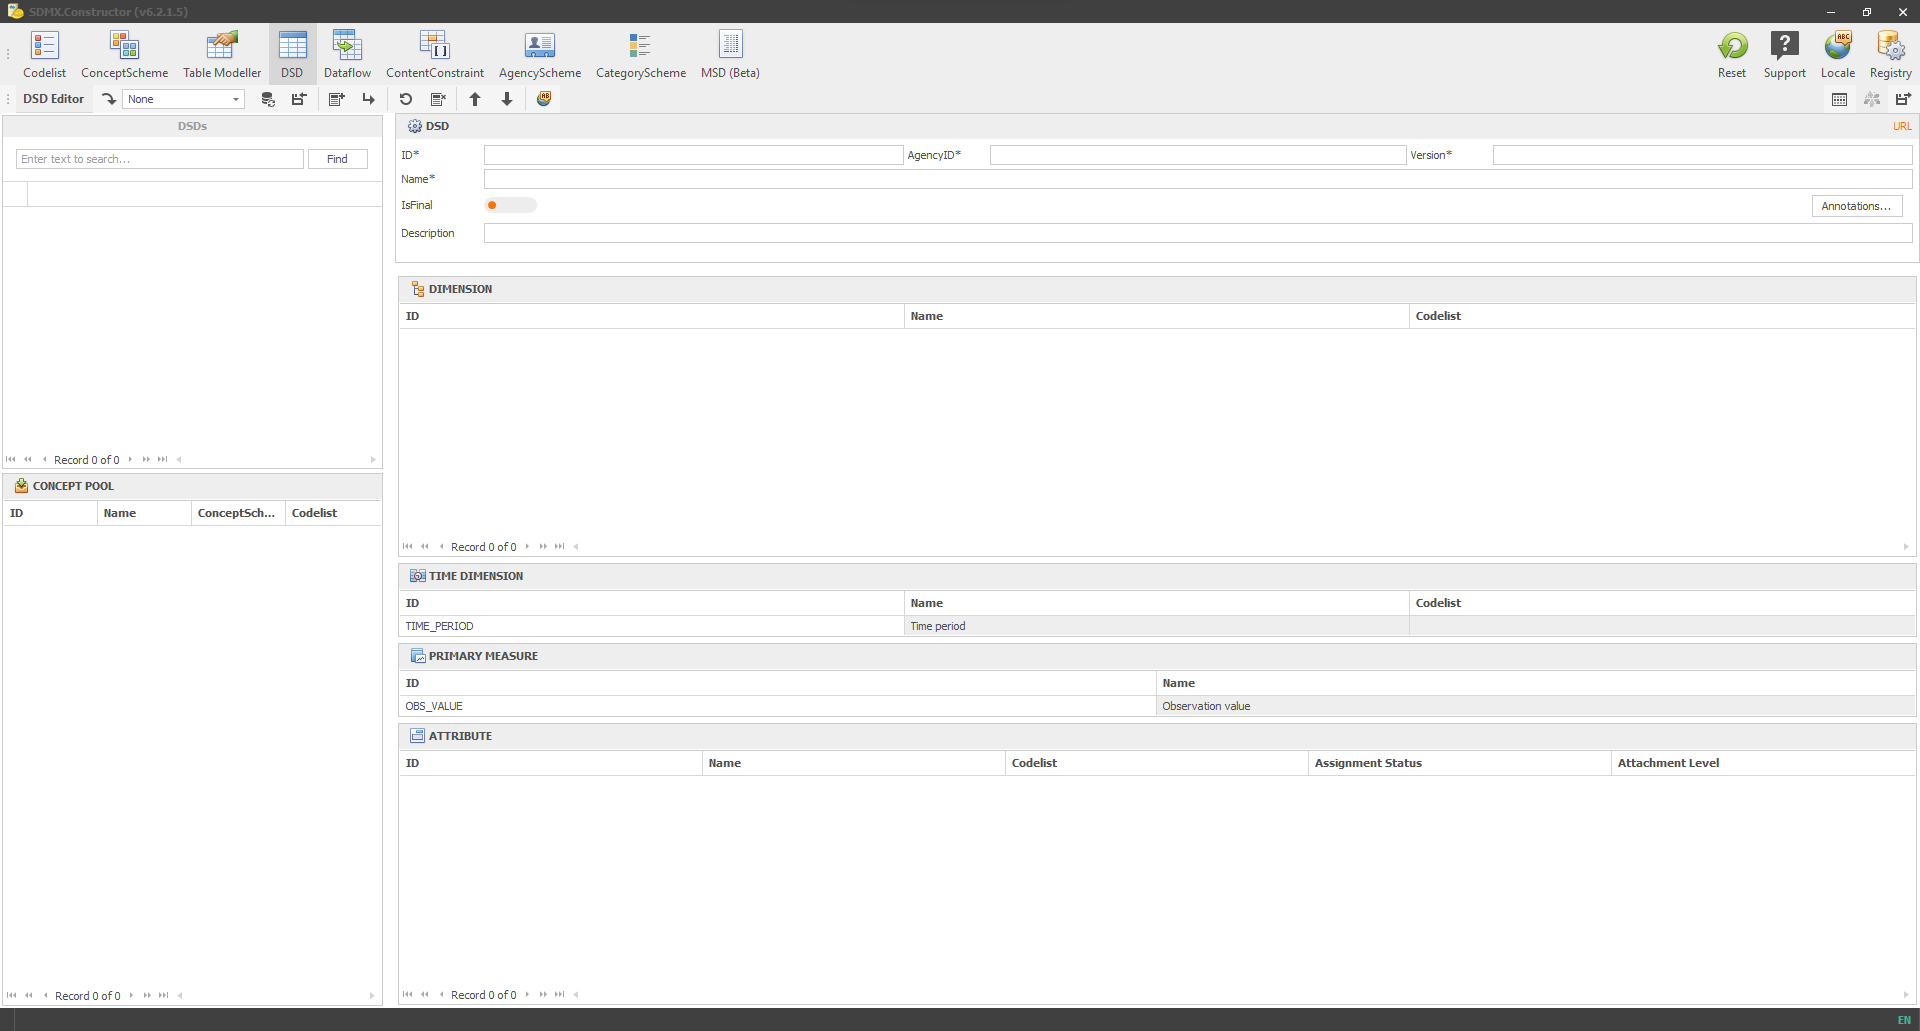
\includegraphics[width=1\linewidth]{./images/image001} \end{center}

\href{images/image001.png}{Click here to enlarge the image}

\hypertarget{audience-and-use-cases}{%
\section*{Audience and use cases}\label{audience-and-use-cases}}
\addcontentsline{toc}{section}{Audience and use cases}

The SDMX Constructor is designed to meet the needs of a wide range of users, from beginners who are new to SDMX to data managers who need advanced capabilities for managing large and complex datasets. In addition to these user types, there may be other groups of users with specific requirements or use cases. This user manual provides guidance and instructions for using the SDMX Constructor, focusing on the needs of these various user types.

\textbf{SDMX beginners}: These users are new to SDMX and want to use the SDMX Constructor to view, edit, and create new SDMX structural artefacts. They may need assistance understanding the SDMX concepts, terminology, and the software's user interface.

For SDMX beginners, this manual explains using the SDMX Constructor to access, view, edit, and create SDMX structural artefacts from SDMX registries. While one can find information on SDMX concepts and terminology from other sources, this manual focuses explicitly on the user interfaces of the SDMX Constructor. The SDMX beginners may be keen to know how to \protect\hyperlink{accessing-sdmx}{view and access SDMX artefacts from SDMX registries}, as well as how to \protect\hyperlink{connecting-to}{connect to an SDMX registry} through the SDMX Constructor.

\textbf{Data managers}: These users are likely familiar with the SDMX concepts and terminology and may require information about advanced functionalities offered by the SDMX Constructor. For example, they may want to use the SDMX Constructor as a backend client to manage SDMX artefacts for the .Stat Data Lifecycle Manager (DLM). For such cases, they may also use the SDMX Constructor to build the initial structural metadata when creating a new .Stat Suite instance.

There are several topics that data managers may be interested in learning when it comes to creating SDMX artefacts from scratch. Firstly, they may want to start by \protect\hyperlink{setting-up}{setting up a registry as a local folder}. Next, they can \protect\hyperlink{preparing-inputs}{prepare inputs} and create several artefacts, including the \protect\hyperlink{creating-agencyscheme}{AgencyScheme}, \protect\hyperlink{creating-conceptscheme}{ConceptScheme, and Codelist} and the \protect\hyperlink{creating-dsd}{DSD, Dataflow, ContentConstraint, and CategoryScheme}. After creating these artefacts, they may want to learn how to \protect\hyperlink{uploading-xml}{upload the XML file to the Data Lifecycle Manager (DLM)}. Additionally, they may want to know how to \protect\hyperlink{accessing-sdmx}{access SDMX artefacts from SDMX registries} and \protect\hyperlink{connecting-to}{connect to an SDMX registry} for editing SDMX artefacts directly in the DLM.

\textbf{SDMX metadata managers}: These users manage SDMX artefacts and ensure their accuracy and consistency. They may use the SDMX Constructor to model data and modify SDMX structural artefacts, including translating SDMX artefacts in various languages, managing annotations and creating Metadata Structure Definition (MSD).

\hypertarget{scope-and-assumptions}{%
\section*{Scope and assumptions}\label{scope-and-assumptions}}
\addcontentsline{toc}{section}{Scope and assumptions}

This comprehensive manual provides a step-by-step guide on getting started with the software, including installing it and creating and managing SDMX artefacts. The manual includes a detailed overview of the tool's user interfaces, including menu items, navigation, and other essential features. The manual does not, however, delve into the intricacies of the SDMX standard itself. Describing the SDMX standard is beyond the scope of this manual, as it is an extensive and complex topic requiring more in-depth discussion and is available elsewhere. Instead, the manual assumes that readers are familiar with the SDMX standard and focuses on explaining how to use the tool within that context.

\hypertarget{overview}{%
\section*{Overview}\label{overview}}
\addcontentsline{toc}{section}{Overview}

The chapters in this manual build up toward providing comprehensive guidance that covers topics users need to know to get started with the application, understand its navigation, and use its features and functionalities to model data effectively. The manual includes the following chapters.

\begin{itemize}
\tightlist
\item
  Chapter 1: \protect\hyperlink{benefits-of}{Benefits of SDMX Constructor}
\item
  Chapter 2: \protect\hyperlink{getting-started}{Getting Started}
\item
  Chapter 3: \protect\hyperlink{user-interface}{User Interface}
\item
  Chapter 4: \protect\hyperlink{using-sdmx}{Using SDMX Constructor}
\item
  Chapter 5: \protect\hyperlink{special-topics}{Special Topics}
\end{itemize}

\hypertarget{contact-information}{%
\section*{Contact information}\label{contact-information}}
\addcontentsline{toc}{section}{Contact information}

For more information and to seek basic technical assistance or support on the tool, please reach out International Labour Organization - Department of Statistics at \href{mailto:sdmx.support@ilo.org}{\nolinkurl{sdmx.support@ilo.org}}.

\hypertarget{benefits-of}{%
\chapter{Benefits of SDMX Constructor}\label{benefits-of}}

SDMX Constructor is a software tool that offers a range of features and functionalities designed to streamline and optimise the SDMX workflow, making it an essential tool for statistical organisations, data providers, and other stakeholders involved in the production and dissemination of statistical data.

One of the key benefits of SDMX Constructor is that it allows users to access and query SDMX structural artefacts from SDMX registries (through APIs in the background) in a desktop environment. This makes it easy for users to quickly and easily search for and view essential components of SDMX structural metadata, such as Data Structure Definitions (DSDs) and dataflows.

In addition to its API capabilities, SDMX Constructor offers two other essential features. The first is that it helps users model data following the SDMX standards. For example, SDMX Constructor makes it easy for users to define data structures and create data flows following SDMX standards. This is essential for data providers who need easy-to-use tools to ensure that their data can be shared and used by others in a consistent and standardised way.

The second essential feature of SDMX Constructor is that it enables users to create and edit SDMX artefacts in a user-friendly environment. This includes creating and editing code lists, concept schemes, DSDs, dataflows, content constraints, category schemes and Metadata Structure Definitions (MSDs)\footnote{These SDMX terms are detailed in the SDMX Glossary, available on the official SDMX website. The SDMX Glossary is a comprehensive reference guide that provides definitions and explanations for all the key terms and concepts used in SDMX. You can access the SDMX Glossary by visiting the following link: \url{https://sdmx.org/?sdmx_news=sdmx-glossary}.}. SDMX Constructor provides a user-friendly interface that makes it easy for users to create and modify these artefacts without needing to be an expert in SDMX.

Finally, SDMX Constructor supports data availability and access through online data portals. Using SDMX Constructor, data providers can ensure their data is available and accessible through online data portals built on SDMX standards. This allows data users to easily access and use the data they need for their research, analysis, and other activities.

\hypertarget{getting-started}{%
\chapter{Getting Started}\label{getting-started}}

In this chapter, you will find information about the installation process of SDMX Constructor in a Windows environment. Specifically, it will cover the system requirements necessary to install the software, the steps required to download the executable file and the subsequent installation process. The chapter will also explain the software update process, providing practical guidance on keeping your SDMX Constructor current.

\hypertarget{system-requirements}{%
\section{System requirements}\label{system-requirements}}

Before installing any desktop software, ensuring the computer meets the necessary system requirements is essential. These requirements can include hardware specifications like processor speed, memory, and storage capacity, as well as software prerequisites like operating system version and other dependencies. Find below the minimum system requirements for installing and running SDMX Constructor.

\begin{itemize}
\tightlist
\item
  Windows 7 or later in both 32- and 64-bit environments
\item
  .NET 4.5.2 or later with all updates and patches
\item
  200MB disk space for the software
\end{itemize}

\hypertarget{installation}{%
\section{Installation}\label{installation}}

\textbf{Step 1}: Visit the site \url{https://ilostat.github.io/dsdc/} and click on the INSTALL menu option (as shown below).

\begin{center}
\includegraphics[width=1\linewidth]{./images/image003} \end{center}

\textbf{Step 2}: In the resulting page, click on ``here'' (as shown below)

\begin{center}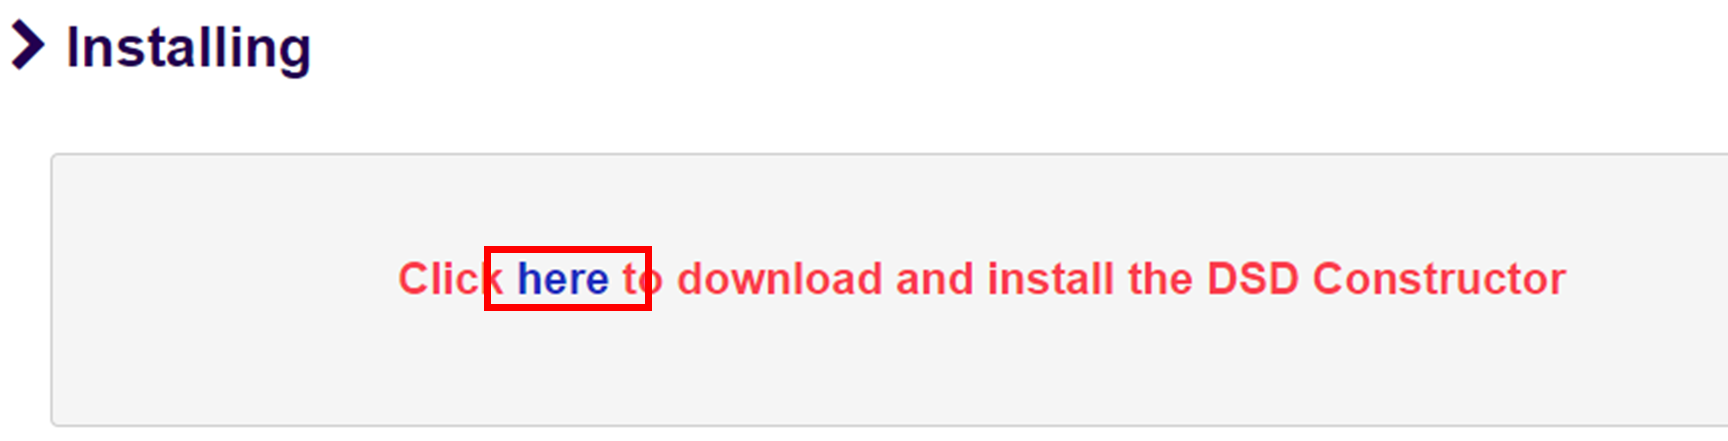
\includegraphics[width=1\linewidth]{./images/image005} \end{center}

\textbf{Step 3}: An interface (as shown below) will open, requiring you to enter a few details (your name, your email, and the name of your organisation (if applicable)).

\begin{center}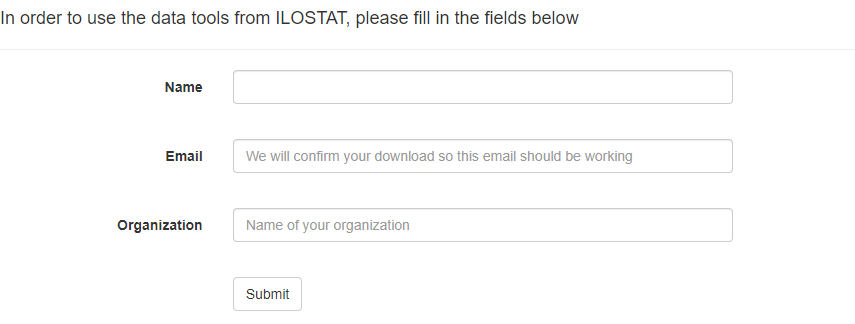
\includegraphics[width=1\linewidth]{./images/image007} \end{center}

\textbf{Step 4}: The download will start when you fill in the form and submit the information. The software installer file, named ``ILOSTAT\_DSD\_Constructor\_Setup.exe'', will be downloaded.

\textbf{Step 5}: Double-click on this file to begin the installation process. Select `Install' on the security message and wait for the installation process to complete.

\hypertarget{software-updates}{%
\section{Software updates}\label{software-updates}}

The SDMX Constructor updates itself to the latest version (if available) using the ClickOnce Deployment technique. This method ensures a streamlined installation process with minimal user involvement. An internet connection is required when launching the application to initiate the update. The software will check for available updates and automatically download and install them in the background without requiring any input from the user. This feature helps to ensure that users always have access to the latest version of the software, with the latest bug fixes, performance improvements, and new features.

\hypertarget{user-interface}{%
\chapter{User Interface}\label{user-interface}}

This chapter will provide you with a comprehensive guide on the main aspects of the SDMX Constructor's user interface. It will cover three main topics. The first topic will be an overview of the user interface, including a detailed explanation of the various menu options and the working area. The second topic will focus on the inputs and outputs of SDMX Constructor. It will cover the different input and output options available. The third topic will provide an overview of the translation functionality in SDMX Constructor.

\hypertarget{general-functions-menu}{%
\section{General Functions Menu}\label{general-functions-menu}}

In the top right corner (as highlighted below), the first group of buttons (General Functions) shows the items applicable to the whole tool. They include Reset, Support, Locale and Registry. See Table 3.1 for a brief overview of the menu items.

\begin{center}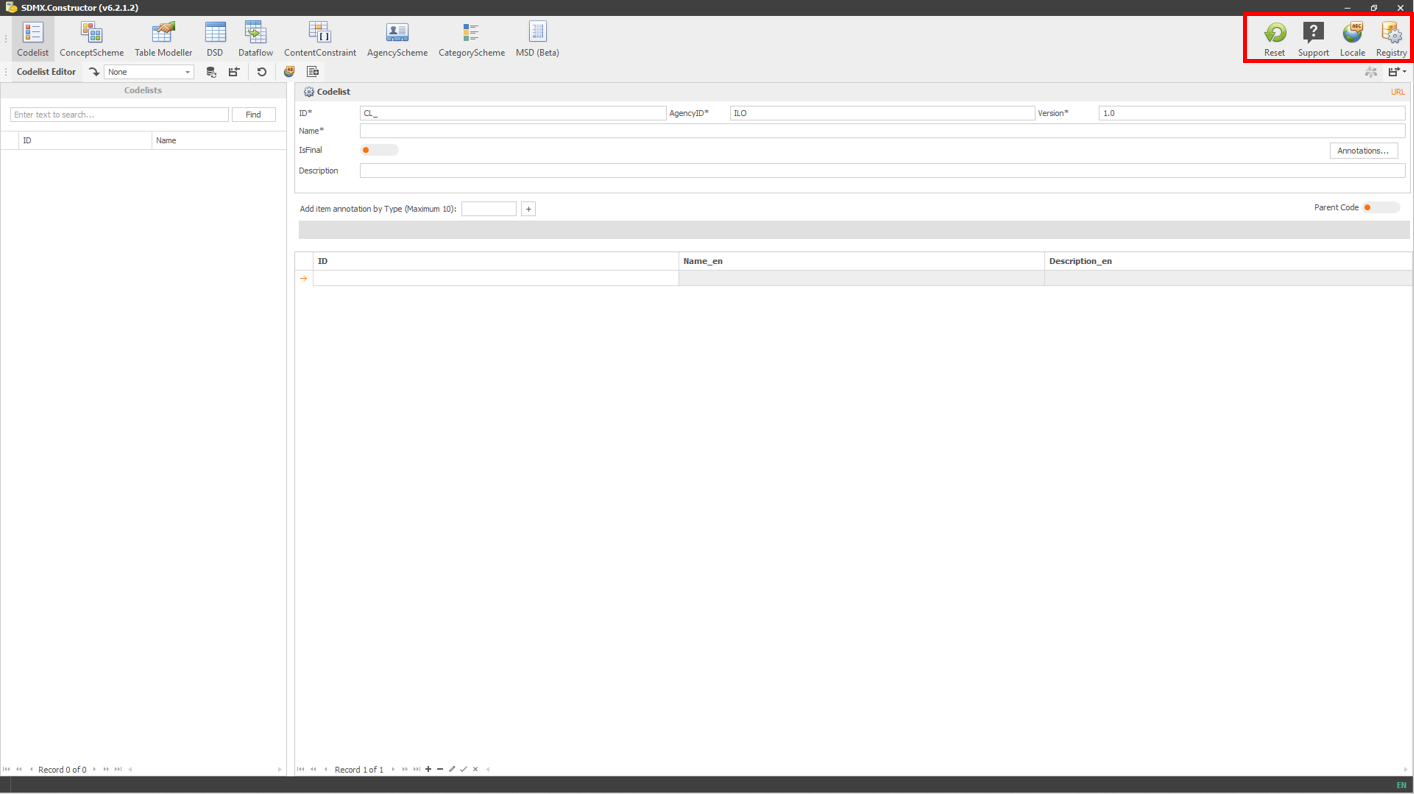
\includegraphics[width=1\linewidth]{./images/image011} \end{center}

\href{images/image011.png}{Click here to enlarge the image}

\begin{longtable}[]{@{}
  >{\raggedright\arraybackslash}p{(\columnwidth - 2\tabcolsep) * \real{0.2917}}
  >{\raggedright\arraybackslash}p{(\columnwidth - 2\tabcolsep) * \real{0.7083}}@{}}
\caption{\label{tab:table31} A bird's-eye view of the menu items in the top right corner (General Functions)}\tabularnewline
\toprule()
\begin{minipage}[b]{\linewidth}\raggedright
Menu item
\end{minipage} & \begin{minipage}[b]{\linewidth}\raggedright
What to expect: A bird's-eye view of General Functions
\end{minipage} \\
\midrule()
\endfirsthead
\toprule()
\begin{minipage}[b]{\linewidth}\raggedright
Menu item
\end{minipage} & \begin{minipage}[b]{\linewidth}\raggedright
What to expect: A bird's-eye view of General Functions
\end{minipage} \\
\midrule()
\endhead
\textbf{Reset} & The Reset button resets the tool to its default settings. It removes all the inputs and initiates a fresh start. \\
\textbf{Support} & The Support button launches the default email application on a computer, with a new email message addressed to the support team for the tool, ready to be composed and sent. \\
\textbf{Locale} & The Support button launches the default email application on a computer, with a new email message addressed to the support team for the tool, ready to be composed and sent. \\
\textbf{Registry} & The Registry button provides several options for users to configure their settings. For example, users can specify the connection details of the SDMX registry (either a local folder or local instance (localhost) or online) and connect with the Data Lifecycle Manager (DLM) component of the .Stat Suite. In addition, the button allows specifying the proxy settings for the internet connection if a proxy is needed. There are also options for entering authentication credentials for automated translation using Google Translation or DeepL API. \\
\bottomrule()
\end{longtable}

\hypertarget{editors-menu}{%
\section{Editors Menu}\label{editors-menu}}

The second group of menu items (Editors) shows the options in the top left corner (as highlighted below). They include Codelist, ConceptScheme, Table Modeller, DSD, Dataflow, ConceptConstraint, AgencyScheme, CategoryScheme and MSD. Each menu item is an entry point for creating and editing a specific artefact. Clicking on any of the options will reveal more particular options below. See Table 3.2 for a brief overview of the menu items (Editors).

\begin{center}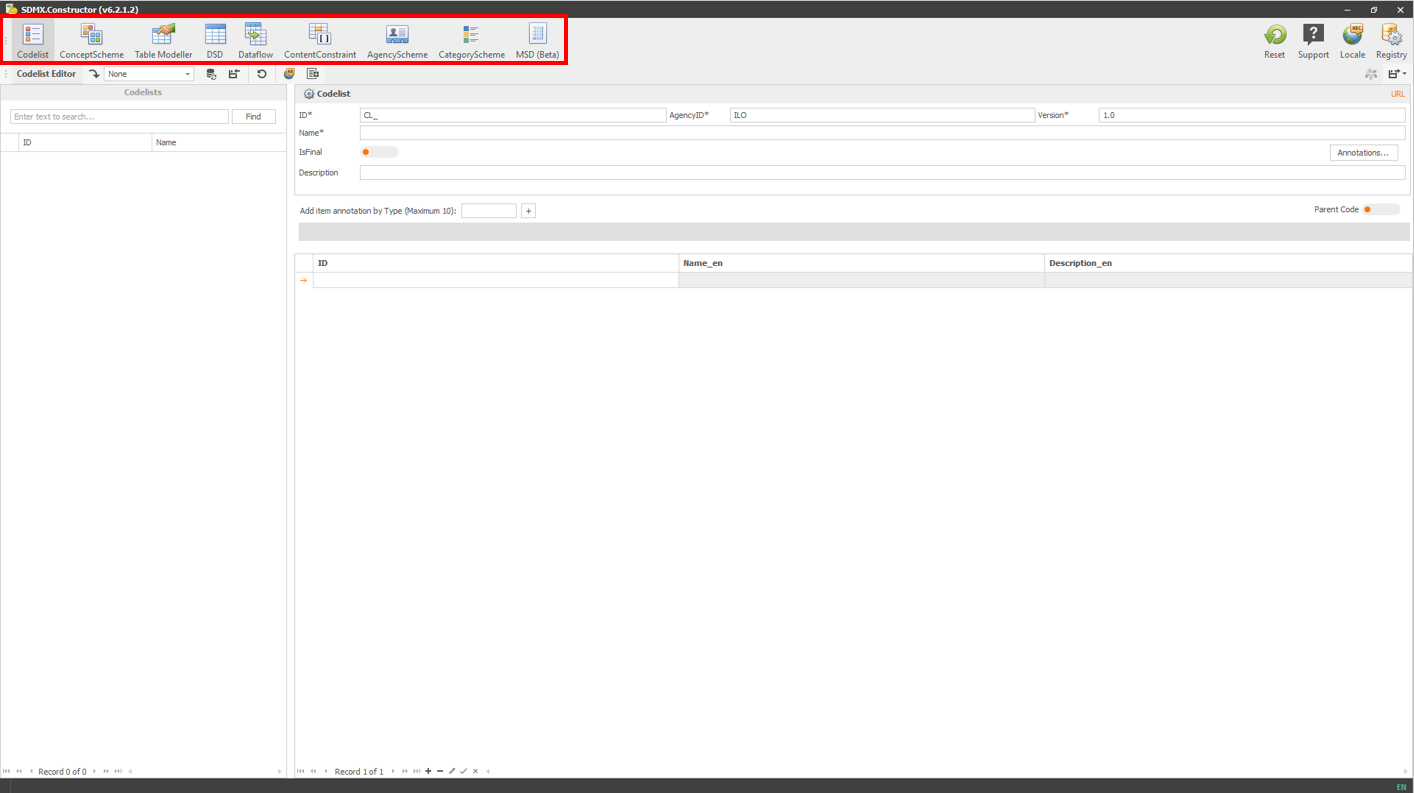
\includegraphics[width=1\linewidth]{./images/image013} \end{center}

\href{images/image013.png}{Click here to enlarge the image}

\begin{longtable}[]{@{}
  >{\raggedright\arraybackslash}p{(\columnwidth - 2\tabcolsep) * \real{0.2917}}
  >{\raggedright\arraybackslash}p{(\columnwidth - 2\tabcolsep) * \real{0.7083}}@{}}
\caption{\label{tab:table32} A bird's-eye view of the menu items in the top left corner (Editors)}\tabularnewline
\toprule()
\begin{minipage}[b]{\linewidth}\raggedright
Menu item
\end{minipage} & \begin{minipage}[b]{\linewidth}\raggedright
What to expect: A bird's-eye view of the menu items in the top left corner (Editors)
\end{minipage} \\
\midrule()
\endfirsthead
\toprule()
\begin{minipage}[b]{\linewidth}\raggedright
Menu item
\end{minipage} & \begin{minipage}[b]{\linewidth}\raggedright
What to expect: A bird's-eye view of the menu items in the top left corner (Editors)
\end{minipage} \\
\midrule()
\endhead
\textbf{Codelist} & The Codelist button shows an interface to create or edit the list of Concepts (dimensions/attributes of a modelled dataset), each having a list of possible values or codes. The codes have unique IDs and (multilingual) labels and may have other information such as order and hierarchy. \\
\textbf{ConceptScheme} & The ConceptScheme button shows an interface to create or edit the Concepts (dimensions/attributes of a modelled dataset). Each concept has an ID and (multilingual) labels and may have other information. \\
\textbf{Table Modeller} & The Table Modeller button shows the options to generate the SDMX artefacts by recreating the statistical table using the Concepts (dimensions/attributes of a modelled data set) with an intuitive user interface (drag and drop). \\
\textbf{DSD} & The DSD button abbreviating Data Structure Definition shows an interface to create or edit the structure of a modelled dataset. It specifies the dimensions, attributes and their possible values or codes. \\
\textbf{Dataflow} & The Dataflow button shows an interface to create or edit a subset and representation of a DSD and describes which dimensions to show on rows or columns. \\
\textbf{ConceptConstraint} & The ConceptConstraint button shows an interface to create or edit combinations of codes that are allowed for various artefacts of the dataflows. \\
\textbf{AgencyScheme} & The AgencyScheme button shows an interface to create or edit a hierarchical list of agencies or organisations. Each agency or organisation is identified by a unique code (ID), a name, and other descriptive information. \\
\textbf{CategoryScheme} & The CategoryScheme button shows an interface to create or edit a CategoryScheme, which is essentially a list of categories organised in a hierarchical structure. Each category is identified by a unique code (ID), a name, and other descriptive information. \\
\textbf{MSD} & The MSD button abbreviating Metadata Structure Definition shows an interface describing the structure of reference metadata associated with a data set. It specifies the elements and attributes that can be used to represent metadata concepts and the relationships between them. \\
\bottomrule()
\end{longtable}

\hypertarget{editor-ribbon-menu}{%
\section{Editor Ribbon Menu}\label{editor-ribbon-menu}}

The third group of menu items (Editor Ribbon) are in the top left corner and below the second group of menu items (as highlighted below).

\begin{center}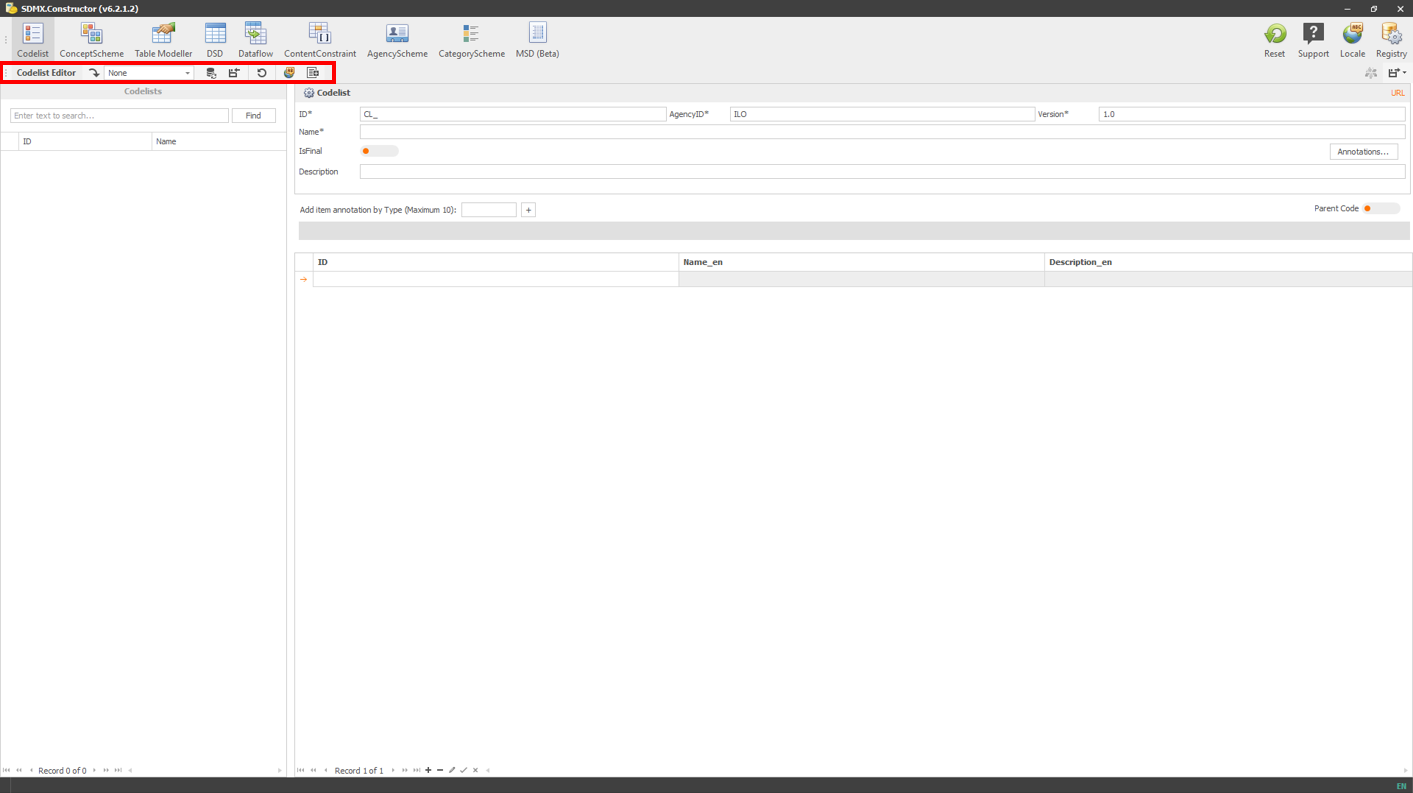
\includegraphics[width=1\linewidth]{./images/image015} \end{center}

\href{images/image015.png}{Click here to enlarge the image}

It contains icons that represent the most commonly used features of the selected options above, and hovering over each icon will reveal a tooltip that describes its function. The options available in this group of menu items change according to the menu item selected on the top menu.

Below are the icons representing the menu items (Editor Ribbon) and their functions. Users can change the size of these icons by right-clicking on any of them, selecting Customize, and selecting the appropriate setting in Options.

\begin{longtable}[]{@{}
  >{\raggedright\arraybackslash}p{(\columnwidth - 2\tabcolsep) * \real{0.2917}}
  >{\raggedright\arraybackslash}p{(\columnwidth - 2\tabcolsep) * \real{0.7083}}@{}}
\caption{\label{tab:table33} A bird's-eye view of the menu items in the Editor Ribbon}\tabularnewline
\toprule()
\begin{minipage}[b]{\linewidth}\raggedright
Menu item
\end{minipage} & \begin{minipage}[b]{\linewidth}\raggedright
Names and functions
\end{minipage} \\
\midrule()
\endfirsthead
\toprule()
\begin{minipage}[b]{\linewidth}\raggedright
Menu item
\end{minipage} & \begin{minipage}[b]{\linewidth}\raggedright
Names and functions
\end{minipage} \\
\midrule()
\endhead

\includegraphics{images/image017.png} & Load from Registry. Select from a dropdown list to load. \\

\includegraphics{images/image019.png} & Refresh the registry. \\

\includegraphics{images/image020.png} & Import. Allows to import an SDMX XML file locally. \\

\includegraphics{images/image021.png} & Reset the current Editor inputs. \\

\includegraphics{images/image022.png} & Translation Service. Provide inline translations for names and descriptions via translation API or manually if needed. \\

\includegraphics{images/image023.png} & Collapse DSDs. \\

\includegraphics{images/image024.png} & Bulk load. Allows to upload multiple items (if available) by copying and pasting. \\

\includegraphics{images/image026.png} & Add New Concept (e.g., Agency or Category). Depending on which Editor is active, e.g., it can help add a new agency if it is for AgencyScheme. \\
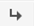
\includegraphics{images/image027.png} & Load Concept. \\

\includegraphics{images/image028.png} & Delete Selected Concepts. \\

\includegraphics{images/image030.png} & Move Up. \\

\includegraphics{images/image031.png} & Move Down. \\
\bottomrule()
\end{longtable}

If a user chooses ``Codelist'' from the top menu, the corresponding menu items in the third group will appear as ``Load from registry'' (from the dropdown menu), ``Refresh the registry'', ``Import'', ``Reset the current Editor inputs'', ``Translation Service'', and ``Bulk load''.

However, suppose a user selects ``ConceptScheme'' from the top menu instead. In that case, the user will see three additional options: ``Add New Concept'', ``Load Concept'', and ``Delete Selected Concepts'' relevant to the chosen menu item at the top, i.e., ``ConceptScheme''.

All options available within this menu group per the item selected on the top menu are listed below.

\begin{center}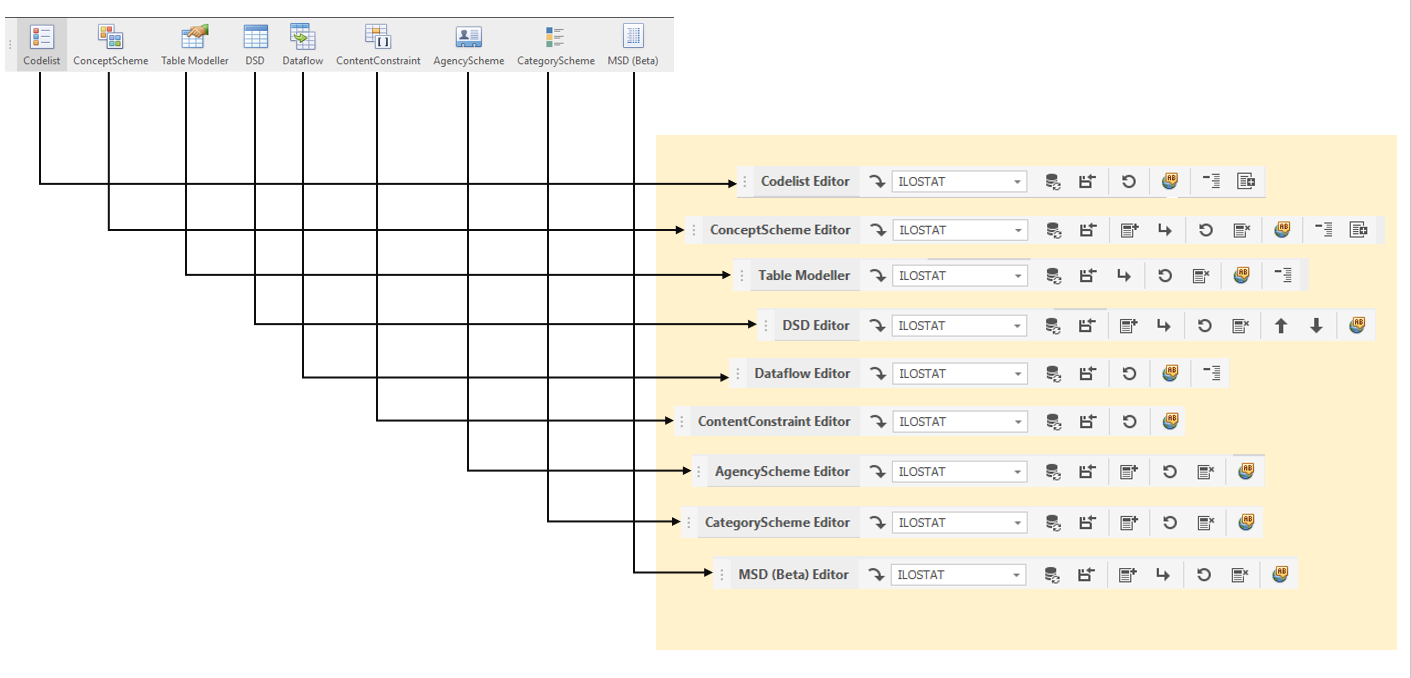
\includegraphics[width=1\linewidth]{./images/image032} \end{center}

\href{images/image032.png}{Click here to enlarge the image}

\hypertarget{preview-and-export-menu}{%
\section{Preview and Export Menu}\label{preview-and-export-menu}}

The fourth menu item group (Preview and Export) is in the top right corner and below the first group of menu items (as highlighted below).

\begin{center}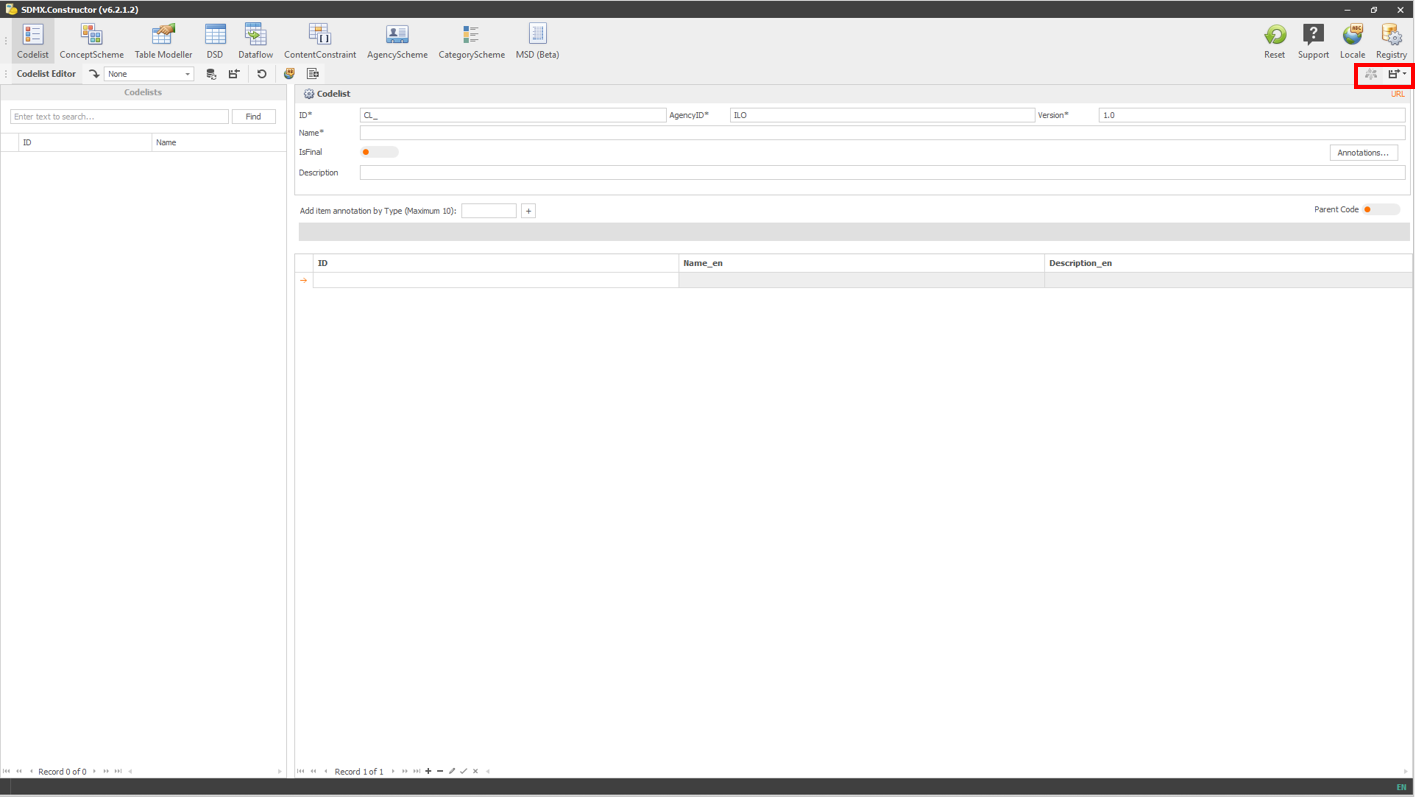
\includegraphics[width=1\linewidth]{./images/image034} \end{center}

\href{images/image034.png}{Click here to enlarge the image}

The options available in this group of menu items are related to the preview and export functionalities of the tool and change according to the menu item selected on the top menu (the second group of menu items (Editors)).

Below are the icons representing the menu items, along with their features. Users can change the size of these icons by right-clicking on any of them, selecting Customize, and selecting the appropriate setting in Options.

\begin{longtable}[]{@{}
  >{\raggedright\arraybackslash}p{(\columnwidth - 2\tabcolsep) * \real{0.2917}}
  >{\raggedright\arraybackslash}p{(\columnwidth - 2\tabcolsep) * \real{0.7083}}@{}}
\caption{\label{tab:table34} A bird's-eye view of the menu items in the Editor Ribbon}\tabularnewline
\toprule()
\begin{minipage}[b]{\linewidth}\raggedright
Menu item
\end{minipage} & \begin{minipage}[b]{\linewidth}\raggedright
Names and functions
\end{minipage} \\
\midrule()
\endfirsthead
\toprule()
\begin{minipage}[b]{\linewidth}\raggedright
Menu item
\end{minipage} & \begin{minipage}[b]{\linewidth}\raggedright
Names and functions
\end{minipage} \\
\midrule()
\endhead

\includegraphics{images/image036.png} & Export. It saves the SDMX artefact in a local folder. It is available for DSD, Dataflow, ContentConstraint, AgencyScheme, and MSD without specific options. However, options are available to save artefacts from: 1. Codelist (available in the following formats: .Stat v7 Dim, CSV and SDMX-ML) and 2. ConceptScheme, Table Modeller and CategoryScheme (available in two flavours: Save with descendants and Save without descendants). \\

\includegraphics{images/image037.png} or 
\includegraphics{images/image038.png} & Push to DLM (DLM is short for Data Lifecycle Manager of the .Stat Suite). This icon becomes active (appears with colours) when the tool is connected with a DLM instance. It is available for Codelist, DSD, Dataflow, ContentConstraint, AgencyScheme, and MSD without specific options. However, options are available to save artefacts from ConceptScheme, Table Modeller and CategoryScheme. \\

\includegraphics{images/image039.png} & Structure Viewer. It lets you preview the tabulation and download the MS Excel and CSV templates. It is available for DSD and Dataflow. \\
\bottomrule()
\end{longtable}

\hypertarget{working-area}{%
\section{Working area}\label{working-area}}

The following section explains the working area of the tool.

Below the menu items on top, the user interface appears divided into two main parts. First, the left pane on the interface serves as a space to hold the artefacts' list. The other side is designated to showcase relevant details (both sides are highlighted in different colours in the screenshot below). Selecting (by double-clicking) an artefact from the left pane prompts its details to appear on the screen's right-side pane. This layout is available for Codelist, Dataflow and ContentConstraint.

\begin{center}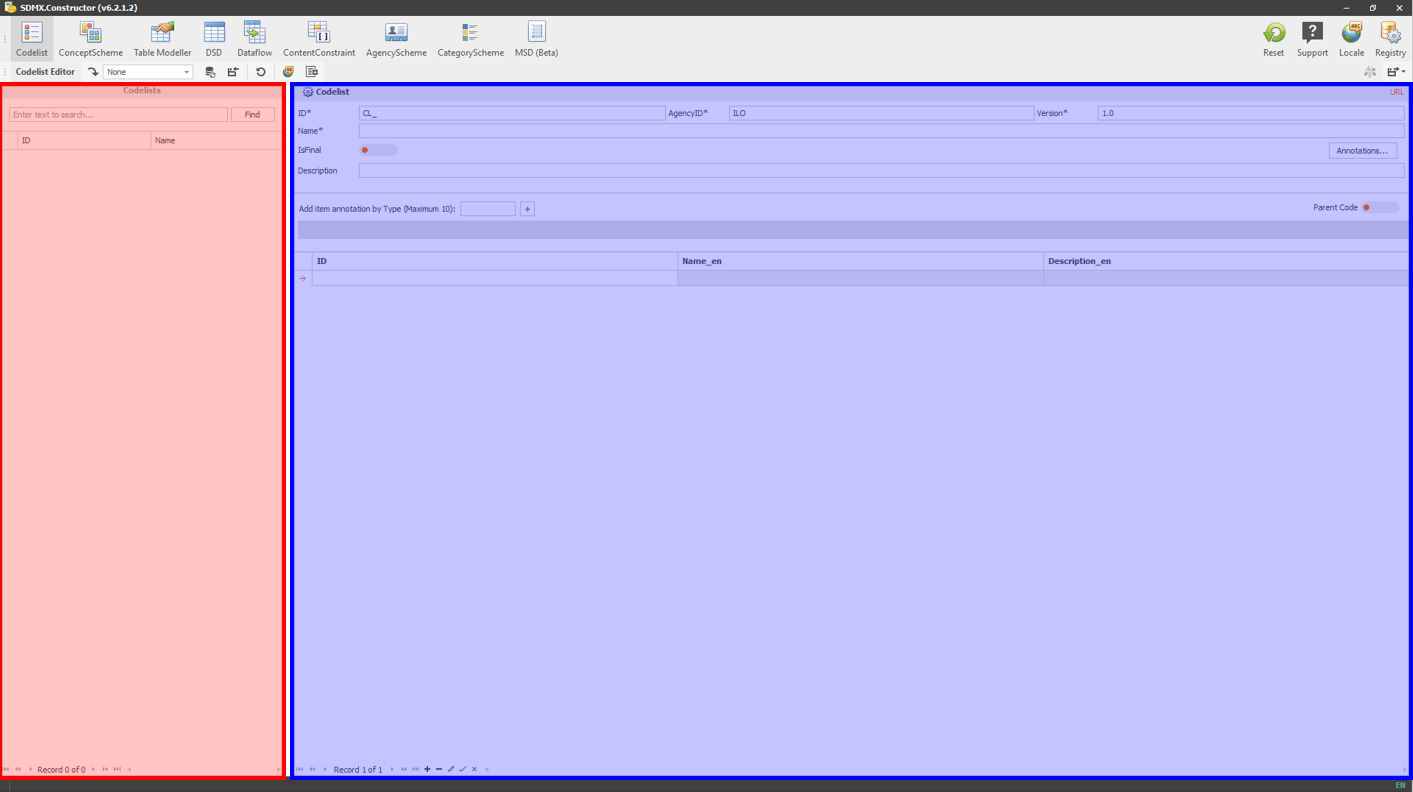
\includegraphics[width=1\linewidth]{./images/image040} \end{center}

\href{images/image040.png}{Click here to enlarge the image}

For ConceptScheme, Table Modeller, DSD, AgencyScheme, CategoryScheme, and MSD, an additional pane also appears in the user interface (below the placeholder for listing the artefacts - (as highlighted below)), which acts as a staging area (or a pool). It becomes a CONCEPTS POOL for ConceptScheme, Table Modeller, DSD and MSD options. And it turns into an AGENCY POOL for AgencyScheme and a CATEGORY POOL for CategoryScheme options.

The users can drag the artefacts back and forth between the pool area and the pane on the right.

\begin{center}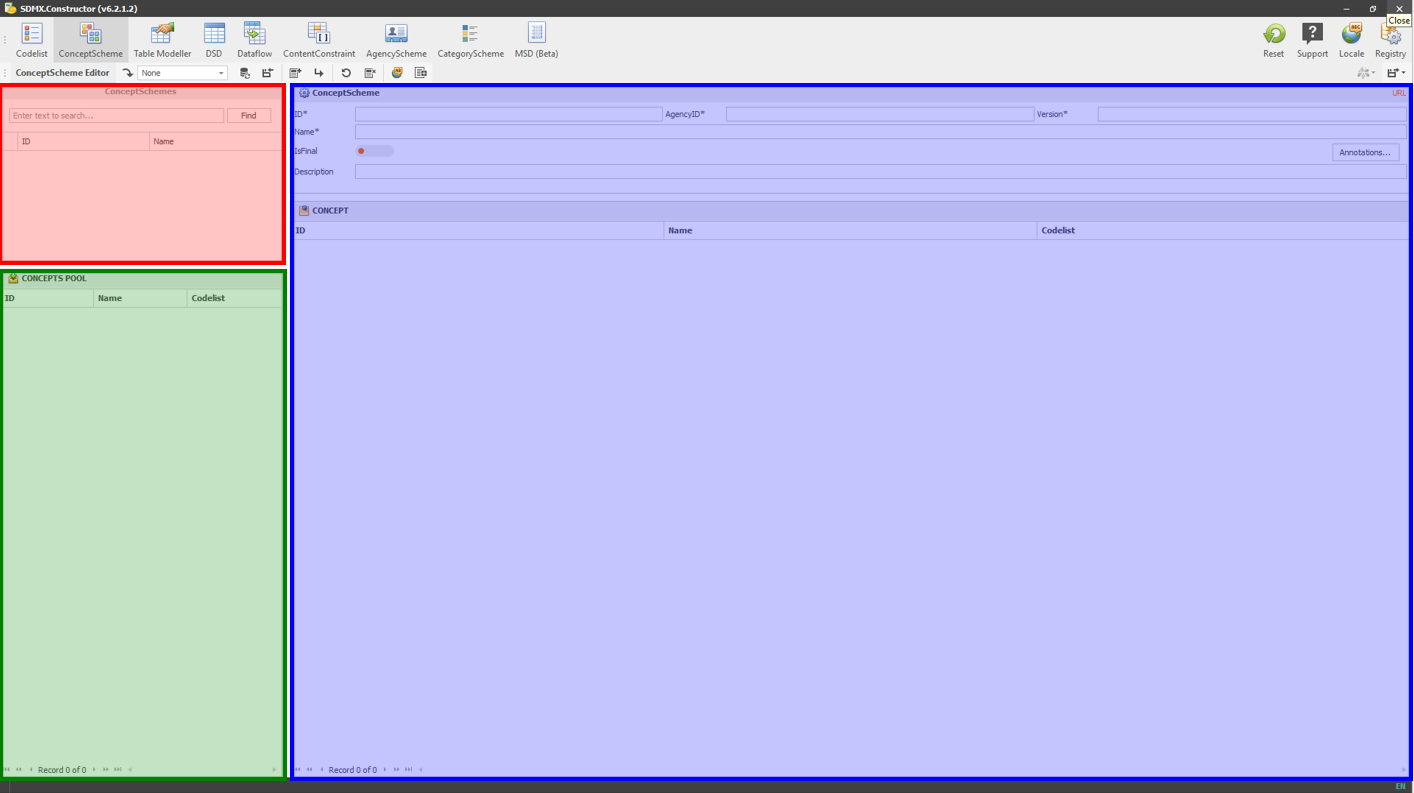
\includegraphics[width=1\linewidth]{./images/image042} \end{center}

\href{images/image042.png}{Click here to enlarge the image}

\hypertarget{input-and-output-methods}{%
\section{Input and output methods}\label{input-and-output-methods}}

Users can input information into SDMX Constructor in several ways, depending on the specific scenarios. The following are the options.

\begin{itemize}
\tightlist
\item
  Typing and copy-pasting: Users can enter information by typing text or copying and pasting into fields in the forms using a keyboard.
\item
  Clicking: Users can interact with buttons, links, menus, or other graphical elements by clicking with a mouse, touchpad, or touchscreen. For example, double-clicking an artefact from the left pane load its details on the screen's right-side pane.
\item
  Dragging and dropping: Users can manipulate objects or select multiple items by dragging and dropping them with a mouse, touchpad, or touchscreen.
\item
  Loading from online SDMX Registry: Users can access pre-prepared SDMX artefacts from many default online SDMX registries. The input method allows users to retrieve information from the SDMX registry.
\end{itemize}

SDMX Constructor presents information to users in a standardised and user-friendly way, using a combination of graphical elements, form-based input and validation and error messages.

\begin{itemize}
\tightlist
\item
  Graphical interface: The DSD Constructor uses a graphical user interface (GUI) that allows users to interact with the metadata components using visual elements like buttons, menus, and icons. This makes it easy for users to navigate and manipulate the metadata and get a quick overview of the SDMX artefacts.
\item
  Form-based input: The DSD Constructor uses form-based input screens to allow users to enter information about the metadata components. The forms are designed to be intuitive and easy to use, with clear labels, dropdown menus, and text boxes that guide users through the input process.
\item
  Validation and error messages: The DSD Constructor validates the metadata components to ensure that they conform to the SDMX standard and are consistent with other components. If there are errors or inconsistencies, the tool provides error messages that help users identify and correct the issues.
\end{itemize}

\hypertarget{translation}{%
\section{Translation}\label{translation}}

DSD Constructor allows users to manage multilingual metadata components easily. Users can choose from automatic or manual translation methods and edit translations using translation tables. The tool simplifies the translation process with standardised language codes and automation and helps users achieve accurate, high-quality translations.

Here are some ways the tool can support the translation of SDMX artefacts:

\begin{itemize}
\tightlist
\item
  Translation into three languages: The tool supports translating content into three languages of your choice. It helps by following two automatic methods, but you can always do it manually if required.
\item
  Automatic translation methods: Using the Google Translate API key, you can connect with Google's translation services. Another automated way is using DeepL. The SDMX Constructor allows programmatic access to DeepL's machine translation technology, bringing high-quality translation capabilities directly to the tool.
\item
  Translation tables: Using these API keys, the SDMX Constructor provides translation tables, which allow users to edit suggested translations of metadata components in different languages. You can enter translations for different language codes, and the tool will automatically populate the translations in the appropriate fields.
\item
  Standardised language codes: The SDMX Constructor uses standardised language codes; users can select from a list of pre-defined language codes.
\end{itemize}

\hypertarget{using-sdmx}{%
\chapter{Using SDMX Constructor}\label{using-sdmx}}

Welcome to the chapter on using SDMX Constructor! This chapter will cover three key topics that will help you make the most of this powerful tool.

The first topic we will cover is how to use SDMX Constructor to access SDMX artefacts from SDMX registries. This will include step-by-step instructions on how to use the tool to connect to a registry, browse its contents, and download the artefacts you need.

Next, we will dive into how to use SDMX Constructor to create new SDMX artefacts from scratch. Whether you need to create a new concept scheme, code list or DSD, SDMX Constructor provides a simple and intuitive interface to help you get the job done.

Finally, we will explore how to use SDMX Constructor to work with .Stat Suite. This powerful platform is designed to help you analyse, visualise, and disseminate statistical data, and SDMX Constructor is the perfect complement to help you access and work with the SDMX artefacts you need.

By the end of this chapter, you will have a solid understanding of how to use SDMX Constructor to access, create, and work with SDMX artefacts, and you will be well on your way to becoming an expert in this powerful tool. So, let's get started!

\hypertarget{accessing-sdmx}{%
\section{Accessing SDMX artefacts from registries}\label{accessing-sdmx}}

In this section, we will walk you through the process of using SDMX Constructor on your computer to access and view the SDMX artefacts from the SDMX registries. This will enable you to easily browse and download the artefacts you need, for example, from the default registries already available in the SDMX Constructor.

\textbf{Default SDMX registries}

You can use the SDMX Constructor on your computer to access and view the SDMX artefacts from the SDMX registries. By default, SDMX Constructor offers the following registries to access SDMX artefacts: SDMX Global Registry: (\url{https://registry.sdmx.org/}), United Nations Statistics Division (UNSD): (\url{https://data.un.org/WS}), the Italian National Institute of Statistics (ESTAT) and the ILO Department of Statistics (ILOSTAT): (\url{https://www.ilo.org/sdmx/index.html}). You can view these by going to the Registry button and opening the Registry Name dropdown in the SDMX Registry tab, as shown below.

\begin{center}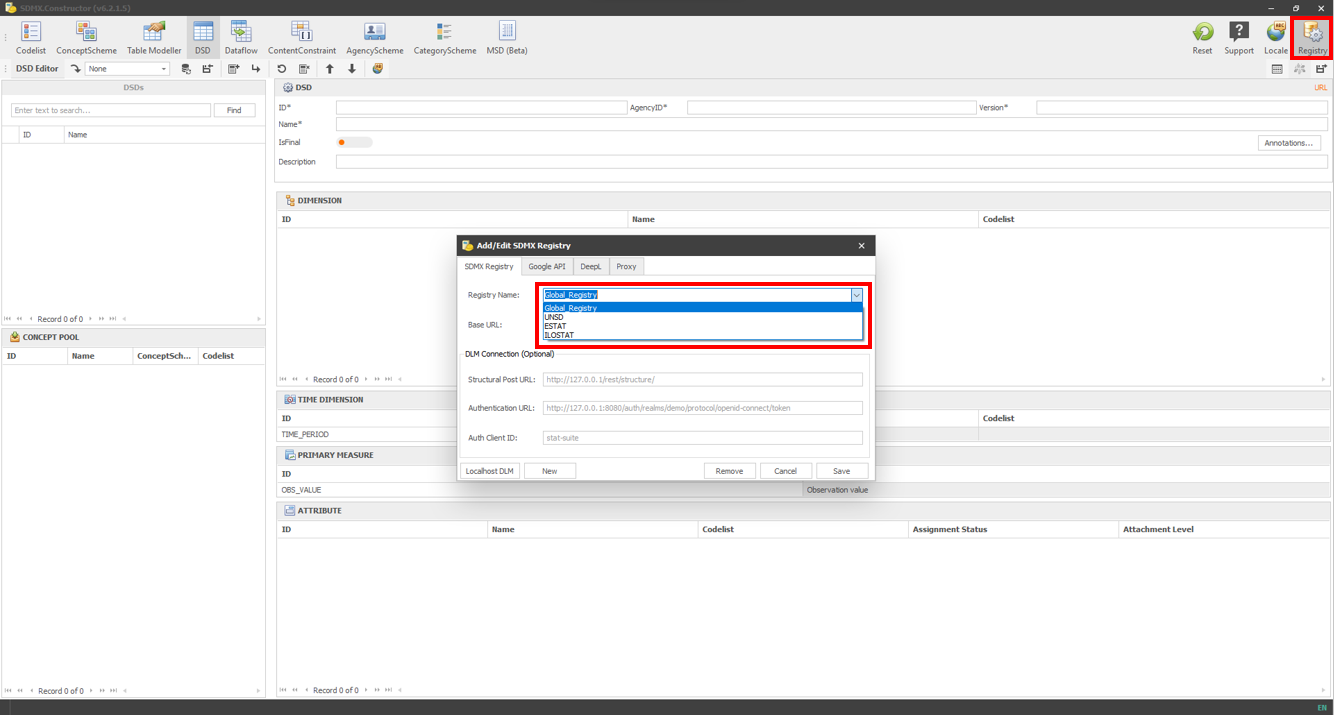
\includegraphics[width=1\linewidth]{./images/image044} \end{center}

\href{images/image044.png}{Click here to enlarge the image}

As shown below, select a registry from the dropdown option to load the artefacts.

\begin{center}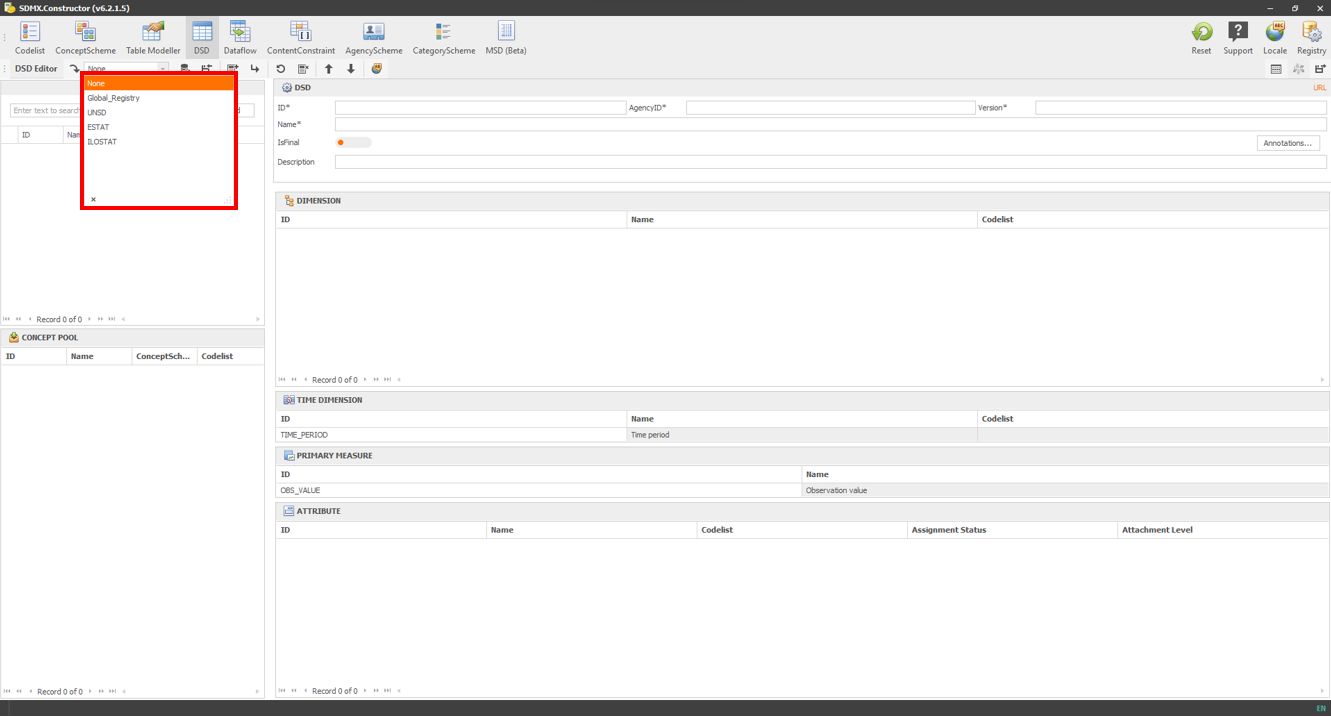
\includegraphics[width=1\linewidth]{./images/image046} \end{center}

\href{images/image046.png}{Click here to enlarge the image}

\hypertarget{setting-up}{%
\section{Setting up a registry as a local folder}\label{setting-up}}

You can use the SDMX Constructor to create SDMX artefacts on your computer without a complicated setup. You can start using it with a local folder on your computer. Following are the steps to set up a registry in a computer's local folder.

\begin{itemize}
\tightlist
\item
  On your computer, create a folder, and let's call it LOCAL\_REGISTRY. The screenshot below shows that the folder is created within the C drive.
\end{itemize}

\begin{center}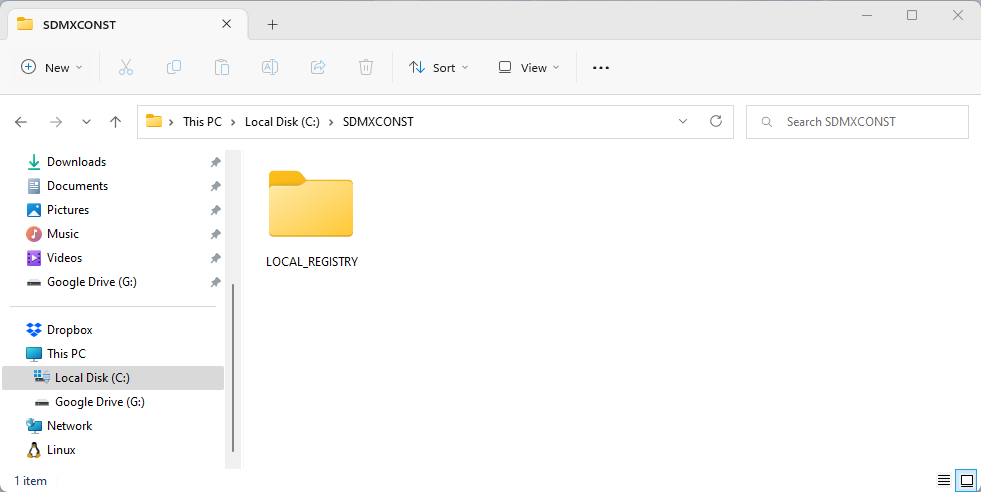
\includegraphics[width=1\linewidth]{./images/image048} \end{center}

\href{images/image048.png}{Click here to enlarge the image}

\begin{itemize}
\tightlist
\item
  Start the SDMX Constructor.
\item
  Click on the Registry button on the SDMX Constructor. It will open a pop-up window showing the default entries in the SDMX Registry tab.
\end{itemize}

\begin{center}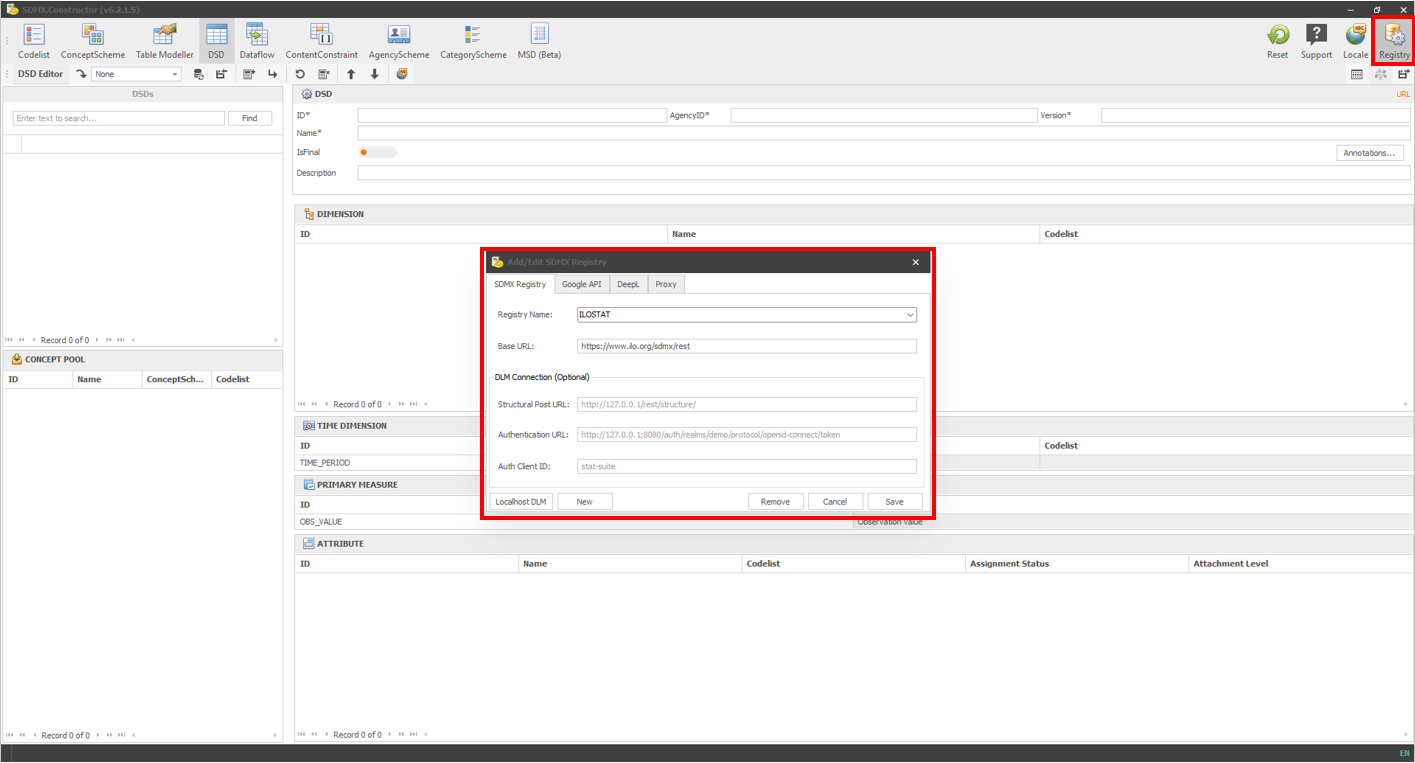
\includegraphics[width=1\linewidth]{./images/image050} \end{center}

\href{images/image050.png}{Click here to enlarge the image}

\begin{itemize}
\tightlist
\item
  In the pop-up window, there are only two fields where we need to make changes: Registry Name and Base URL. You can click the `New' button (which will clear the fields) or type directly within the fields.
\item
  For Registry Name, please type the name of the folder we created before LOCAL\_REGISTRY.
\item
  For the Base URL, get the path of the folder (shown below).
\end{itemize}

\begin{center}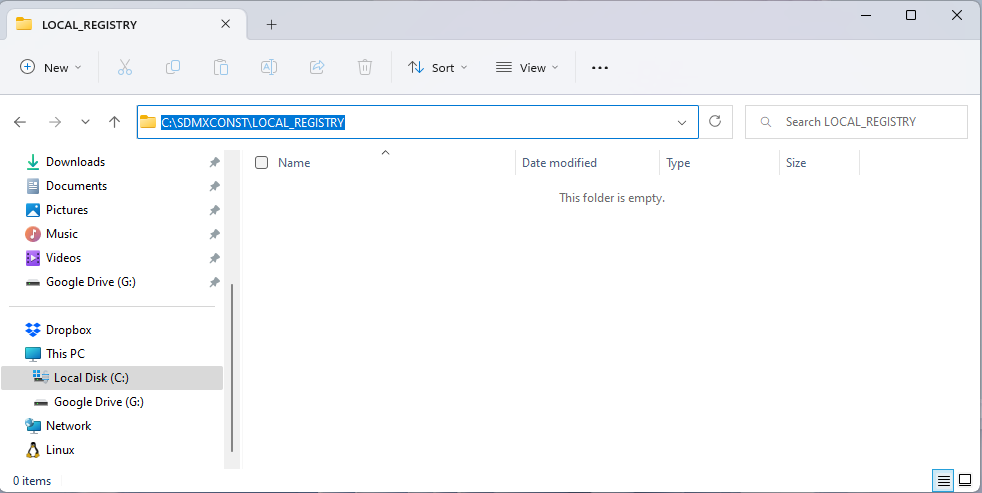
\includegraphics[width=1\linewidth]{./images/image052} \end{center}

\href{images/image052.png}{Click here to enlarge the image}

\begin{itemize}
\tightlist
\item
  After entries in two fields, the pop-up window will look like this:
\end{itemize}

\begin{center}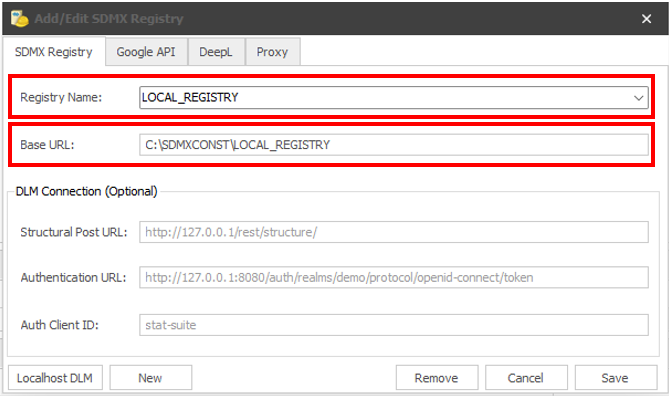
\includegraphics[width=1\linewidth]{./images/image054} \end{center}

\href{images/image054.png}{Click here to enlarge the image}

\begin{itemize}
\tightlist
\item
  Hit Save. It will generate a confirmation message, as shown below.
\end{itemize}

\begin{center}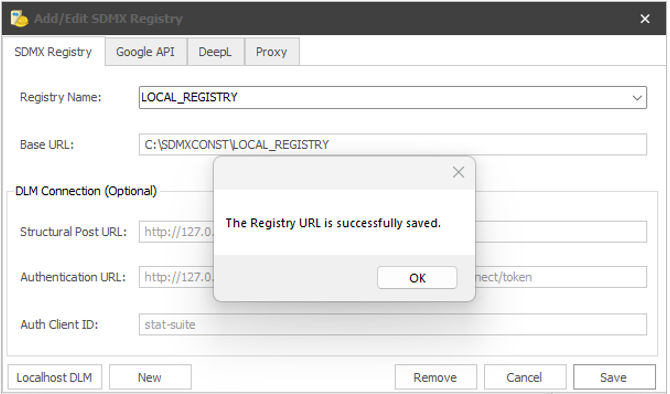
\includegraphics[width=1\linewidth]{./images/image056} \end{center}

\href{images/image056.png}{Click here to enlarge the image}

\begin{itemize}
\tightlist
\item
  Press OK to confirm. The pop-up windows will go away.
\item
  To confirm if the folder is accessible from the tool, in the Editor Ribbon area, if you go to the `Load from registry' option, you will see the LOCAL\_REGISTRY in the dropdown options.
\end{itemize}

\begin{center}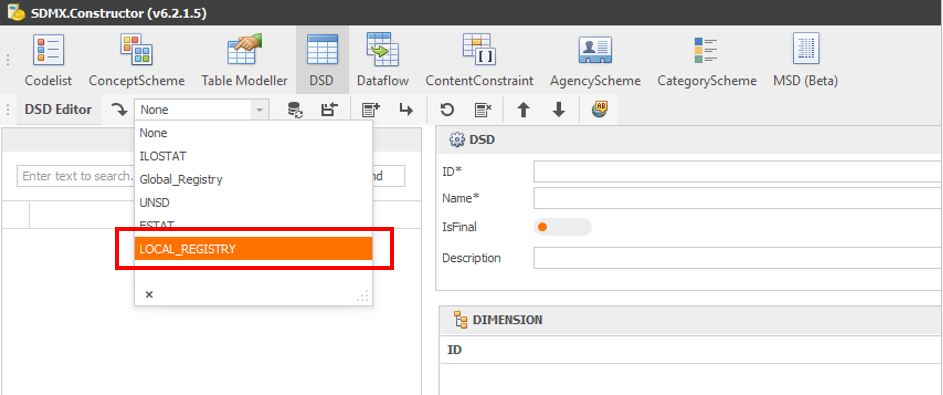
\includegraphics[width=1\linewidth]{./images/image058} \end{center}

\href{images/image058.png}{Click here to enlarge the image}

\begin{itemize}
\tightlist
\item
  The setup with a local folder is complete.
\end{itemize}

\hypertarget{preparing-inputs}{%
\section{Preparing inputs}\label{preparing-inputs}}

To demonstrate the key functionalities of the SDMX Constructor, it is helpful to have a dummy dataset modelled appropriately.

Imagine a country called Demoland and its National Statistical Office (NSO), Demoland NSO. Imagine the Demoland NSO is creating SDMX artefacts for its data in the following two tables.

\begin{longtable}[]{@{}
  >{\raggedright\arraybackslash}p{(\columnwidth - 12\tabcolsep) * \real{0.1835}}
  >{\centering\arraybackslash}p{(\columnwidth - 12\tabcolsep) * \real{0.1009}}
  >{\centering\arraybackslash}p{(\columnwidth - 12\tabcolsep) * \real{0.1284}}
  >{\centering\arraybackslash}p{(\columnwidth - 12\tabcolsep) * \real{0.1743}}
  >{\centering\arraybackslash}p{(\columnwidth - 12\tabcolsep) * \real{0.1101}}
  >{\centering\arraybackslash}p{(\columnwidth - 12\tabcolsep) * \real{0.1284}}
  >{\centering\arraybackslash}p{(\columnwidth - 12\tabcolsep) * \real{0.1743}}@{}}
\caption{\label{tab:table41} Unemployment Rate by sex and region}\tabularnewline
\toprule()
\begin{minipage}[b]{\linewidth}\raggedright
Region
\end{minipage} & \begin{minipage}[b]{\linewidth}\centering
2015
\end{minipage} & \begin{minipage}[b]{\linewidth}\centering
2015
\end{minipage} & \begin{minipage}[b]{\linewidth}\centering
2015
\end{minipage} & \begin{minipage}[b]{\linewidth}\centering
2016
\end{minipage} & \begin{minipage}[b]{\linewidth}\centering
2016
\end{minipage} & \begin{minipage}[b]{\linewidth}\centering
2016
\end{minipage} \\
\midrule()
\endfirsthead
\toprule()
\begin{minipage}[b]{\linewidth}\raggedright
Region
\end{minipage} & \begin{minipage}[b]{\linewidth}\centering
2015
\end{minipage} & \begin{minipage}[b]{\linewidth}\centering
2015
\end{minipage} & \begin{minipage}[b]{\linewidth}\centering
2015
\end{minipage} & \begin{minipage}[b]{\linewidth}\centering
2016
\end{minipage} & \begin{minipage}[b]{\linewidth}\centering
2016
\end{minipage} & \begin{minipage}[b]{\linewidth}\centering
2016
\end{minipage} \\
\midrule()
\endhead
& \textbf{Men} & \textbf{Women} & \textbf{Both Sexes} & \textbf{Men} & \textbf{Women} & \textbf{Both Sexes} \\
Cities and Towns & 14.4 & 20.7 & 17.6 & 14.4 & 21 & 17.2 \\
Urban Villages & 27.8 & 30.3 & 29.1 & 28.2 & 29.4 & 29.1 \\
Rural Areas & 26.2 & 29.6 & 28 & 26.2 & 29.5 & 27.1 \\
Total & 24 & 27.9 & 26 & 24 & 27.9 & 26 \\
\bottomrule()
\end{longtable}

\begin{longtable}[]{@{}lccc@{}}
\caption{\label{tab:table42} Population outside the labour force by sex and age group (2022)}\tabularnewline
\toprule()
Age Group & Men & Women & Both Sexes \\
\midrule()
\endfirsthead
\toprule()
Age Group & Men & Women & Both Sexes \\
\midrule()
\endhead
15-24 & 130,088 & 133,770 & 263,856 \\
25-34 & 33,165 & 60,240 & 93,405 \\
35-44 & 21,970 & 38,944 & 60,914 \\
45-54 & 18,631 & 36,403 & 55,034 \\
55-64 & 26,821 & 44,010 & 70,831 \\
65+ & 45,323 & 78,725 & 124,048 \\
Total & 275,997 & 392,092 & 668,088 \\
\bottomrule()
\end{longtable}

After modelling the data in both tables, we have the following ConceptScheme and Codelist arranged below. Note that the order of the columns in the following tables is per the SDMX Constructor's bulk load default templates (ConceptScheme and Codelist).

\textbf{ConceptScheme:}

\begin{longtable}[]{@{}
  >{\raggedright\arraybackslash}p{(\columnwidth - 6\tabcolsep) * \real{0.1200}}
  >{\raggedright\arraybackslash}p{(\columnwidth - 6\tabcolsep) * \real{0.1680}}
  >{\raggedright\arraybackslash}p{(\columnwidth - 6\tabcolsep) * \real{0.5840}}
  >{\raggedright\arraybackslash}p{(\columnwidth - 6\tabcolsep) * \real{0.1280}}@{}}
\caption{\label{tab:table43} ConceptScheme}\tabularnewline
\toprule()
\begin{minipage}[b]{\linewidth}\raggedright
Concept ID
\end{minipage} & \begin{minipage}[b]{\linewidth}\raggedright
Concept Name
\end{minipage} & \begin{minipage}[b]{\linewidth}\raggedright
Description
\end{minipage} & \begin{minipage}[b]{\linewidth}\raggedright
Codelist ID
\end{minipage} \\
\midrule()
\endfirsthead
\toprule()
\begin{minipage}[b]{\linewidth}\raggedright
Concept ID
\end{minipage} & \begin{minipage}[b]{\linewidth}\raggedright
Concept Name
\end{minipage} & \begin{minipage}[b]{\linewidth}\raggedright
Description
\end{minipage} & \begin{minipage}[b]{\linewidth}\raggedright
Codelist ID
\end{minipage} \\
\midrule()
\endhead
INDICATOR & Indicator & Refers to statistical measure describing a particular aspect of a social, economic or environmental phenomenon & CL\_INDICATOR \\
UNIT\_MEASURE & Unit of measure & Unit in which the observation values are expressed & CL\_UNIT\_MEASURE \\
SEX & Sex & State of being male or female & CL\_SEX \\
GEO & Geographic area & Refers to Urban or Rural locations & CL\_GEO \\
TIME\_PERIOD & Time period & Timespan or point in time to which the observation refers & CL\_TIME\_PERIOD \\
FREQ & Frequency & Time interval at which observations occur over a given time period & CL\_FREQ \\
AGE & Age groups & Length of time that an entity has lived or existed & CL\_AGE \\
OBS\_VALUE & Observation values & Refers to data or observation values & CL\_OBS\_VALUE \\
\bottomrule()
\end{longtable}

\textbf{Codelist:}

\begin{longtable}[]{@{}
  >{\raggedright\arraybackslash}p{(\columnwidth - 6\tabcolsep) * \real{0.1667}}
  >{\raggedright\arraybackslash}p{(\columnwidth - 6\tabcolsep) * \real{0.2188}}
  >{\raggedright\arraybackslash}p{(\columnwidth - 6\tabcolsep) * \real{0.1042}}
  >{\raggedright\arraybackslash}p{(\columnwidth - 6\tabcolsep) * \real{0.5104}}@{}}
\caption{\label{tab:table44} Codelist}\tabularnewline
\toprule()
\begin{minipage}[b]{\linewidth}\raggedright
Codelist ID
\end{minipage} & \begin{minipage}[b]{\linewidth}\raggedright
Concept Name
\end{minipage} & \begin{minipage}[b]{\linewidth}\raggedright
Code ID
\end{minipage} & \begin{minipage}[b]{\linewidth}\raggedright
Code Name
\end{minipage} \\
\midrule()
\endfirsthead
\toprule()
\begin{minipage}[b]{\linewidth}\raggedright
Codelist ID
\end{minipage} & \begin{minipage}[b]{\linewidth}\raggedright
Concept Name
\end{minipage} & \begin{minipage}[b]{\linewidth}\raggedright
Code ID
\end{minipage} & \begin{minipage}[b]{\linewidth}\raggedright
Code Name
\end{minipage} \\
\midrule()
\endhead
CL\_INDICATOR & Indicator & UNER & Unemployment Rate \\
CL\_INDICATOR & Indicator & POLF & Population outside the labour force \\
CL\_UNIT\_MEASURE & Unit of measure & RT & Rate \\
CL\_UNIT\_MEASURE & Unit of measure & PS & Persons \\
CL\_SEX & Sex & M & Men \\
CL\_SEX & Sex & F & Women \\
CL\_SEX & Sex & \_T & Both Sexes (Total) \\
CL\_GEO & Geographical area & M & Cities and Towns (Metropolitan Area) \\
CL\_GEO & Geographical area & U & Urban Villages \\
CL\_GEO & Geographical area & R & Rural Areas \\
CL\_GEO & Geographical area & \_T & Total \\
CL\_FREQ & Frequency & A & Annual \\
CL\_AGE & Age groups & 15T24 & 15-24 \\
CL\_AGE & Age groups & 25T34 & 25-34 \\
CL\_AGE & Age groups & 35T44 & 35-44 \\
CL\_AGE & Age groups & 45T54 & 45-54 \\
CL\_AGE & Age groups & 55T64 & 55-64 \\
CL\_AGE & Age groups & GE65 & 65+ \\
CL\_AGE & Age groups & \_T & Total \\
\bottomrule()
\end{longtable}

We will use these dummy datasets in this user manual to illustrate some critical functionalities of SDMX Constructor.

\hypertarget{creating-agencyscheme}{%
\section{Creating AgencyScheme}\label{creating-agencyscheme}}

\begin{itemize}
\tightlist
\item
  Start the SDMX Constructor, click the AgencyScheme button on top, and select the folder we created before, LOCAL\_REGISTRY, from the AgencyScheme Editor's `Load from registry' dropdown option, as shown below.
\end{itemize}

\begin{center}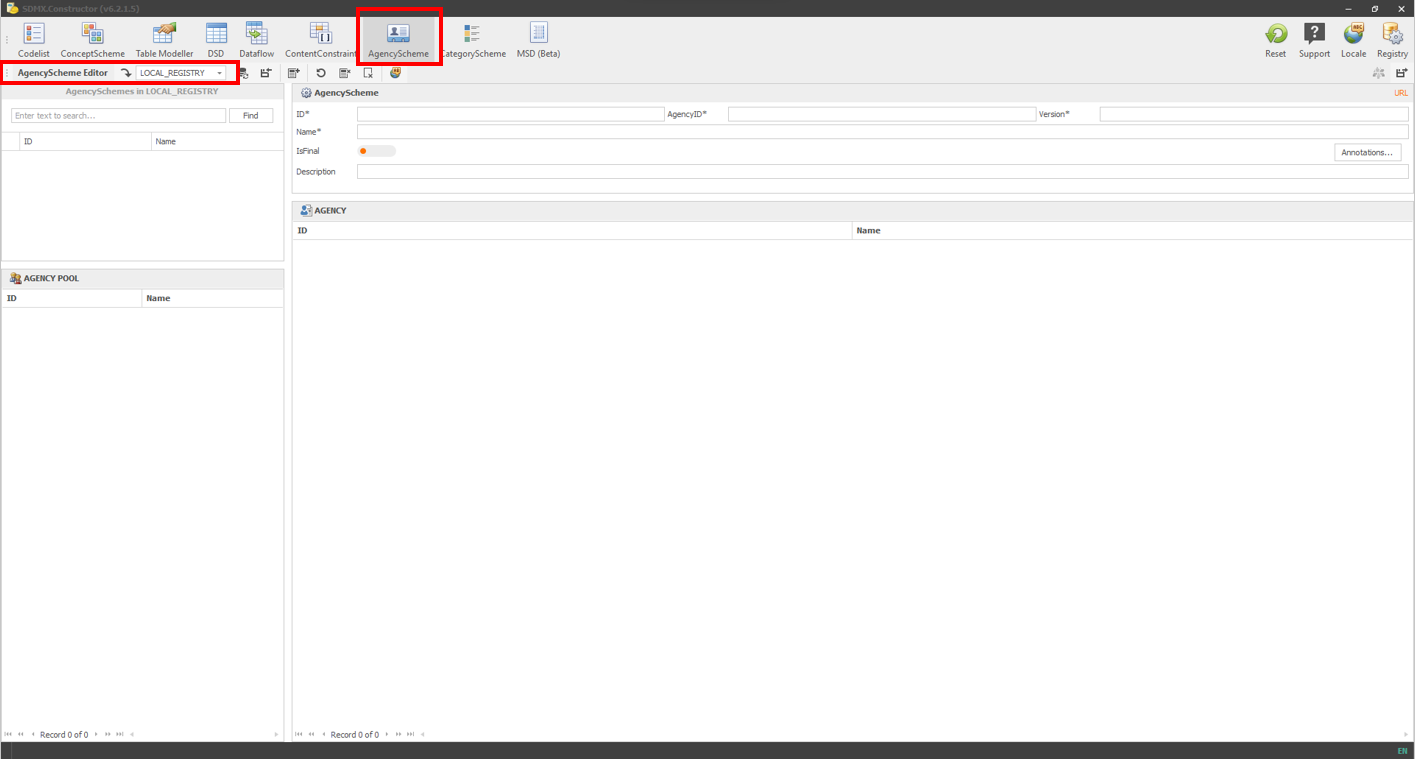
\includegraphics[width=1\linewidth]{./images/image060} \end{center}

\href{images/image060.png}{Click here to enlarge the image}

\begin{itemize}
\tightlist
\item
  Create an AgencyScheme by entering the ID, AgencyID, Version and Name in the fields as shown below. For this exercise, we will have only Demoland NSO as an agency (all data are from Demoland NSO). We will do it in two stages. First, we will enter the properties for the AgencyScheme and then create the agency.
\end{itemize}

\begin{quote}
\textbf{Note on IDs and versions}: All SDMX artefacts, have a unique identifier: In case of AgencySchme these are Agency ID, ID, and Version. Each artefact is assigned a specific version number to keep track of changes and avoid conflicts. This makes sure that the artefacts are managed efficiently and can be easily shared and reused by others while also giving users control over the artefacts they create.
\end{quote}

\begin{itemize}
\tightlist
\item
  For ID, enter AGENCIES; For AgencyID, enter Demoland\_NSO; for version, enter 1.0; and for the Name, enter Demoland NSO Agency Scheme as shown below.
\end{itemize}

\begin{center}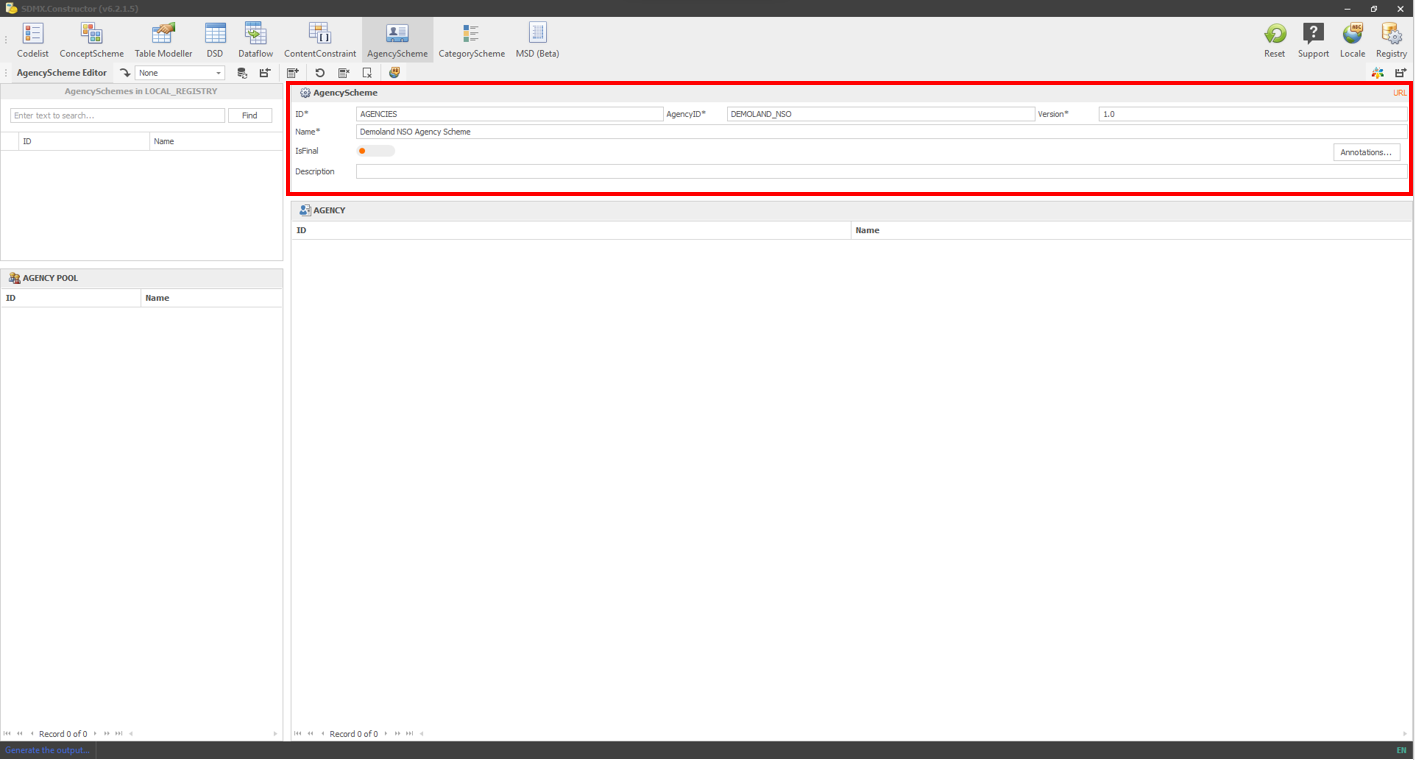
\includegraphics[width=1\linewidth]{./images/image062} \end{center}

\href{images/image062.png}{Click here to enlarge the image}

\begin{itemize}
\tightlist
\item
  Now, we create the agency (as part of the AgencyScheme) by clicking on `Add New Agency' as shown below.
\end{itemize}

\begin{center}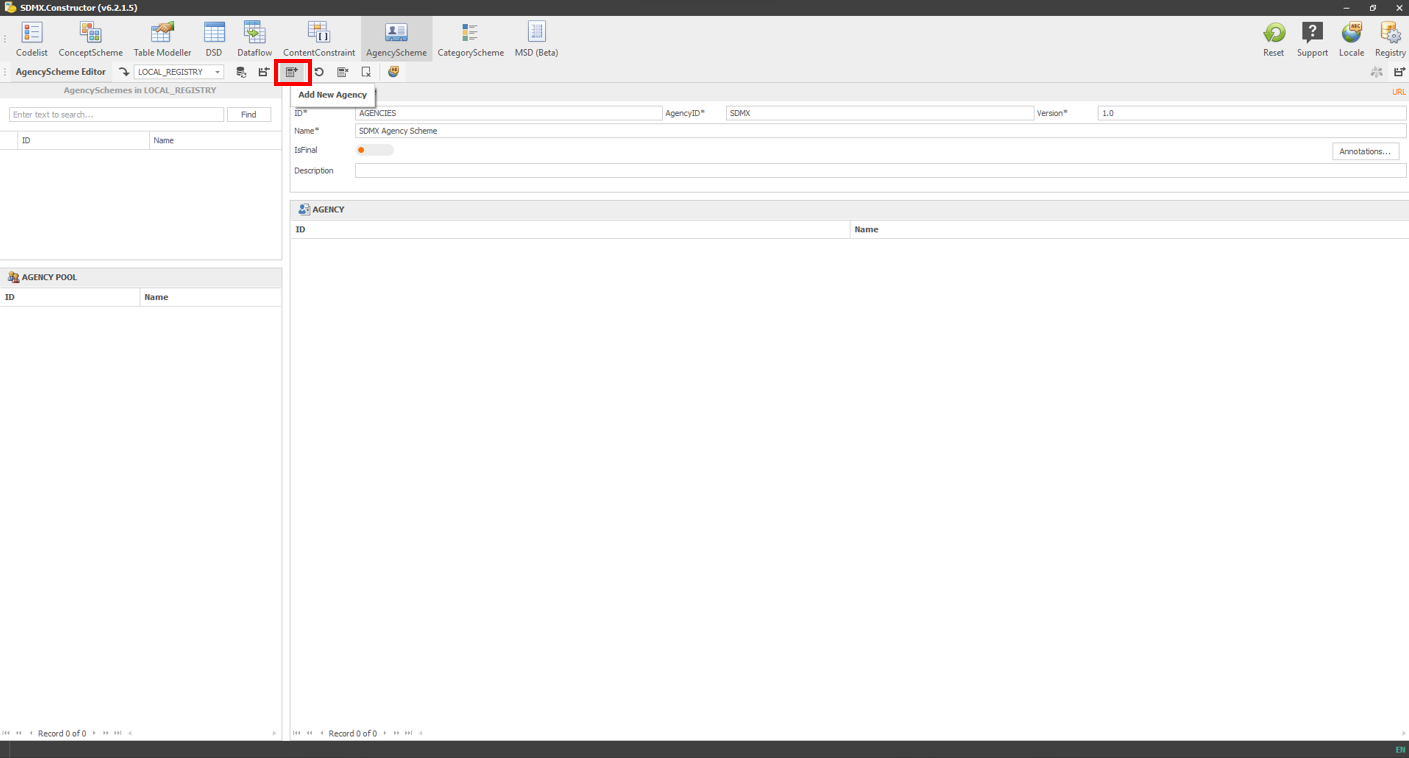
\includegraphics[width=1\linewidth]{./images/image064} \end{center}

\href{images/image064.png}{Click here to enlarge the image}

\begin{itemize}
\tightlist
\item
  Clicking on `Add New Agency' will open a pop-up window. We create the Demoland NSO agency by entering DEMOLAND\_NSO in the ID and Demoland NSO in the Name field in the Add Agency pop-up and clicking Apply (as shown below).
\end{itemize}

\begin{center}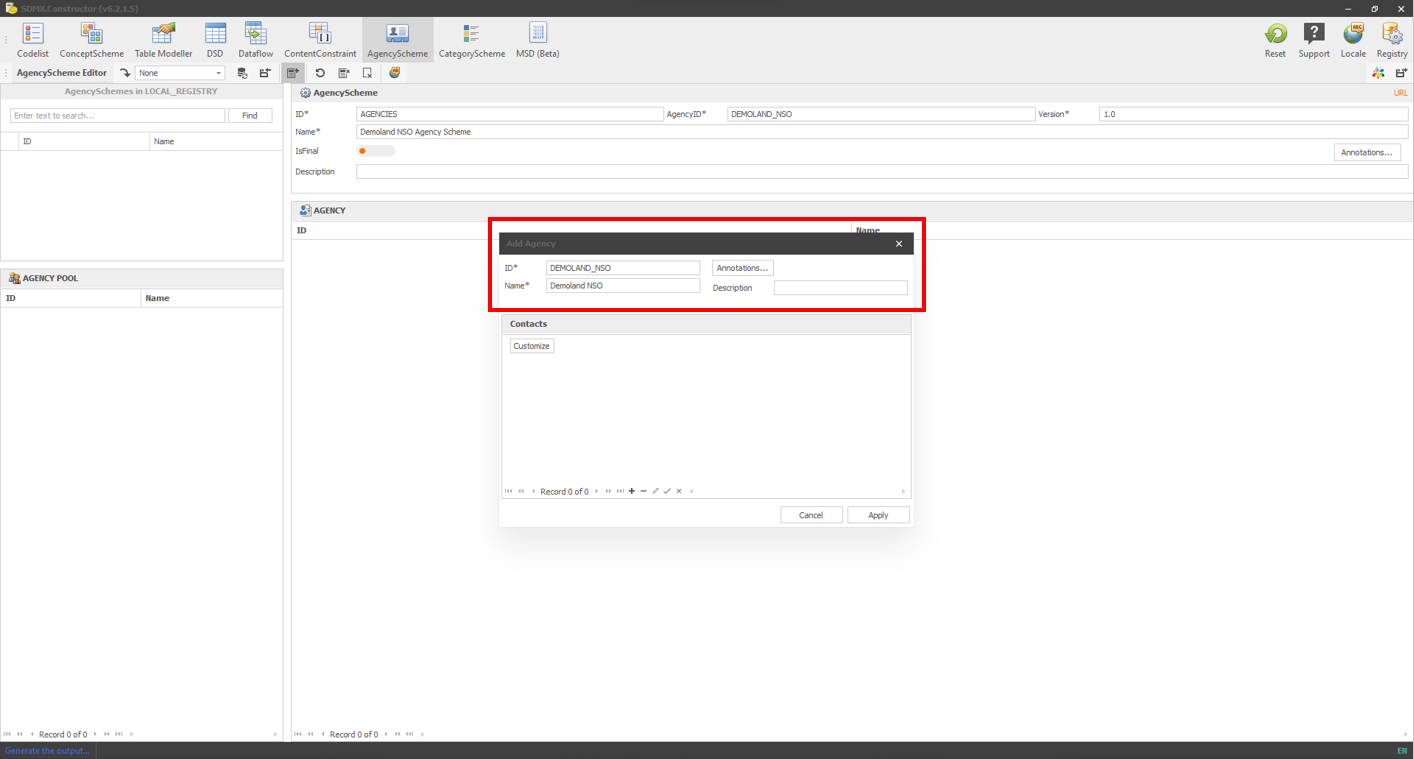
\includegraphics[width=1\linewidth]{./images/image066} \end{center}

\href{images/image066.png}{Click here to enlarge the image}

\begin{itemize}
\tightlist
\item
  Once we finished creating the agency, it would look like the following (the agency will be in the AGENCY POOL).
\end{itemize}

\begin{center}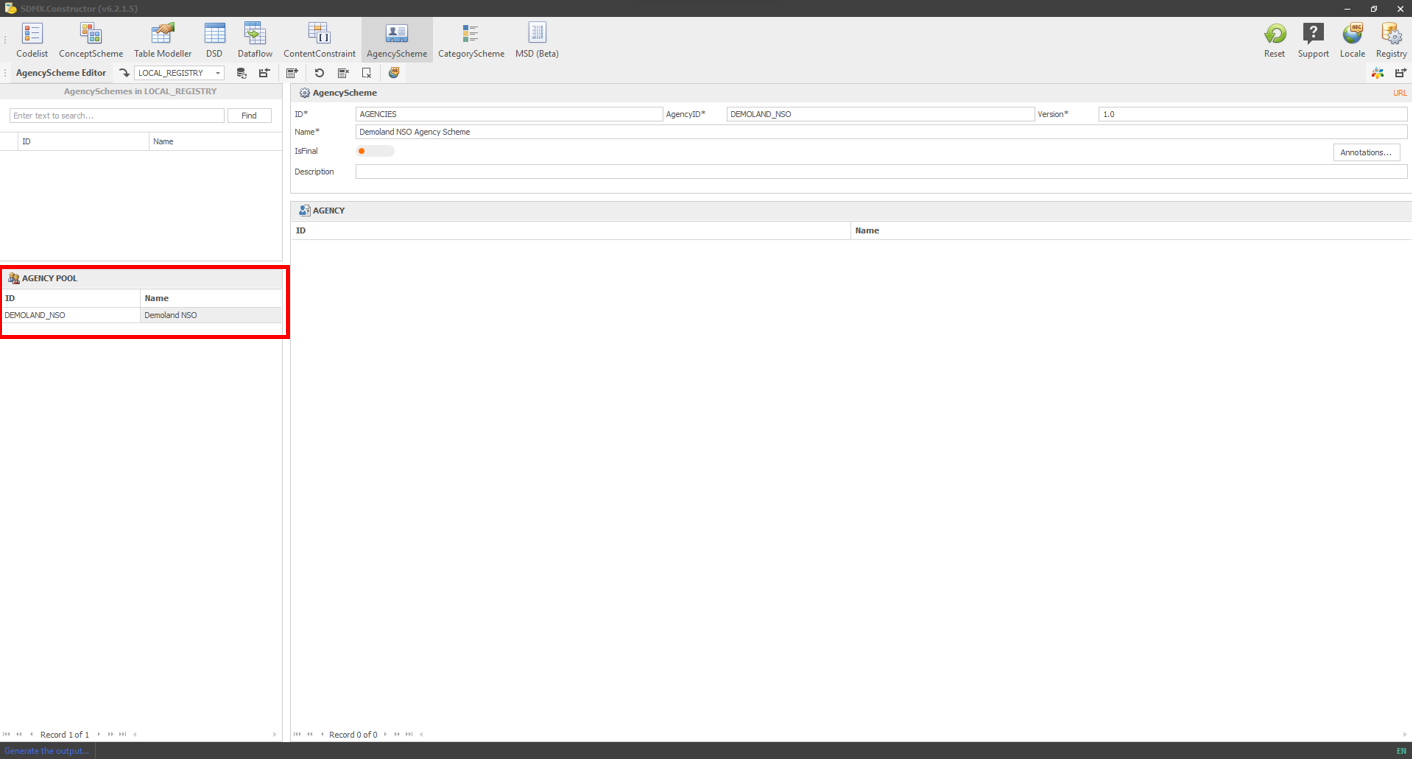
\includegraphics[width=1\linewidth]{./images/image068} \end{center}

\href{images/image068.png}{Click here to enlarge the image}

\begin{itemize}
\tightlist
\item
  Move the agency from the AGENCY POOL to the AGENCY space on the right pane by selecting and dragging it. After the move, it would look like the following.
\end{itemize}

\begin{center}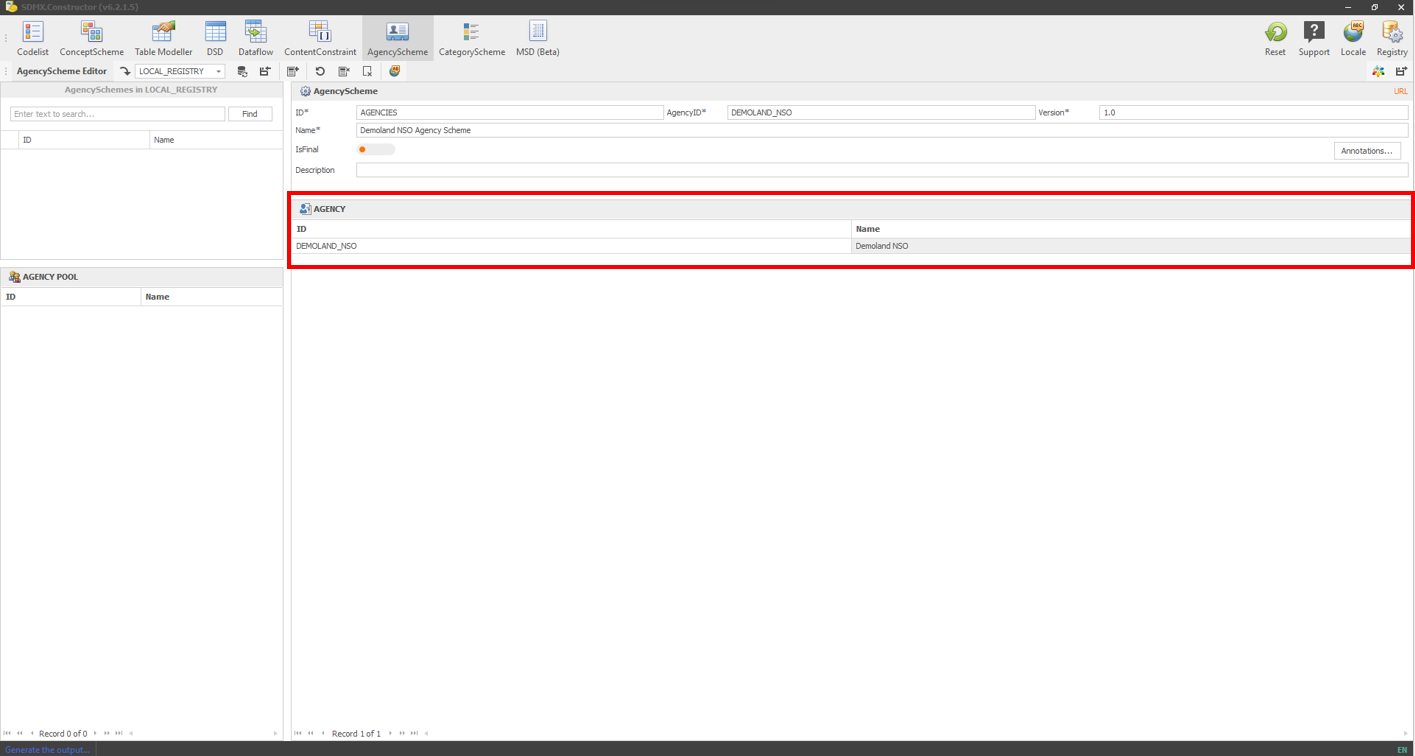
\includegraphics[width=1\linewidth]{./images/image070} \end{center}

\href{images/image070.png}{Click here to enlarge the image}

\begin{itemize}
\tightlist
\item
  Click the Export button highlighted below to save the agency scheme in the folder.
\end{itemize}

\begin{center}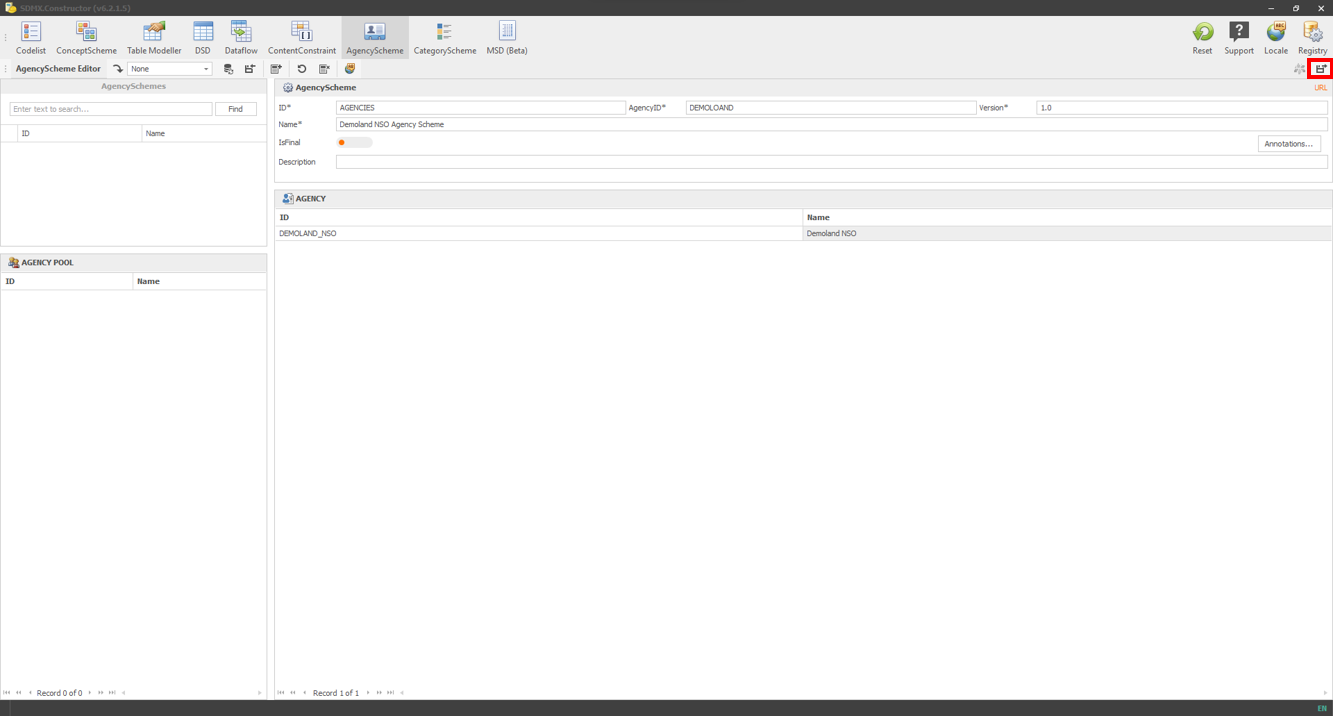
\includegraphics[width=1\linewidth]{./images/image072} \end{center}

\href{images/image072.png}{Click here to enlarge the image}

\begin{itemize}
\tightlist
\item
  As shown below, a pop-up window will open to confirm the saving location.
\end{itemize}

\begin{center}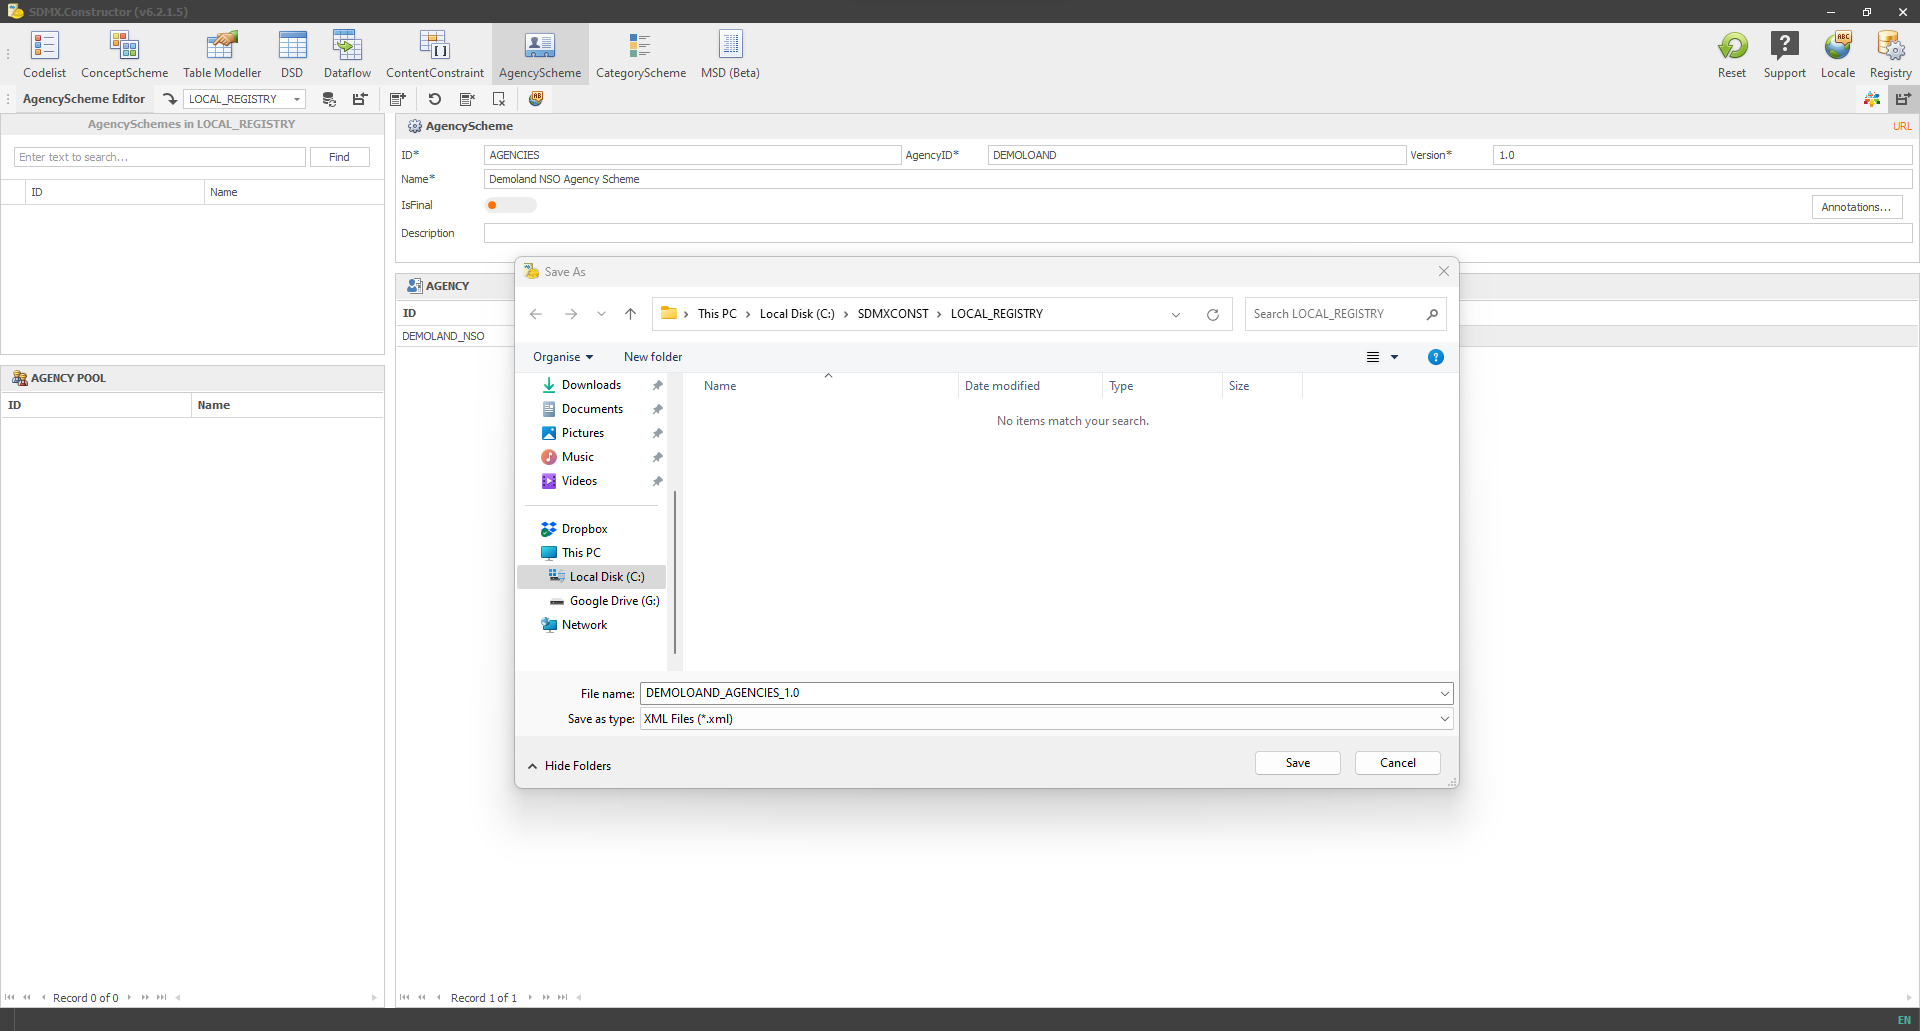
\includegraphics[width=1\linewidth]{./images/image074} \end{center}

\href{images/image074.png}{Click here to enlarge the image}

\begin{itemize}
\tightlist
\item
  Clicking on Save will prompt another message (``All files in this directory (path) with delete and merged into a single file (path) are you sure to continue?''), as shown below.
\end{itemize}

\begin{center}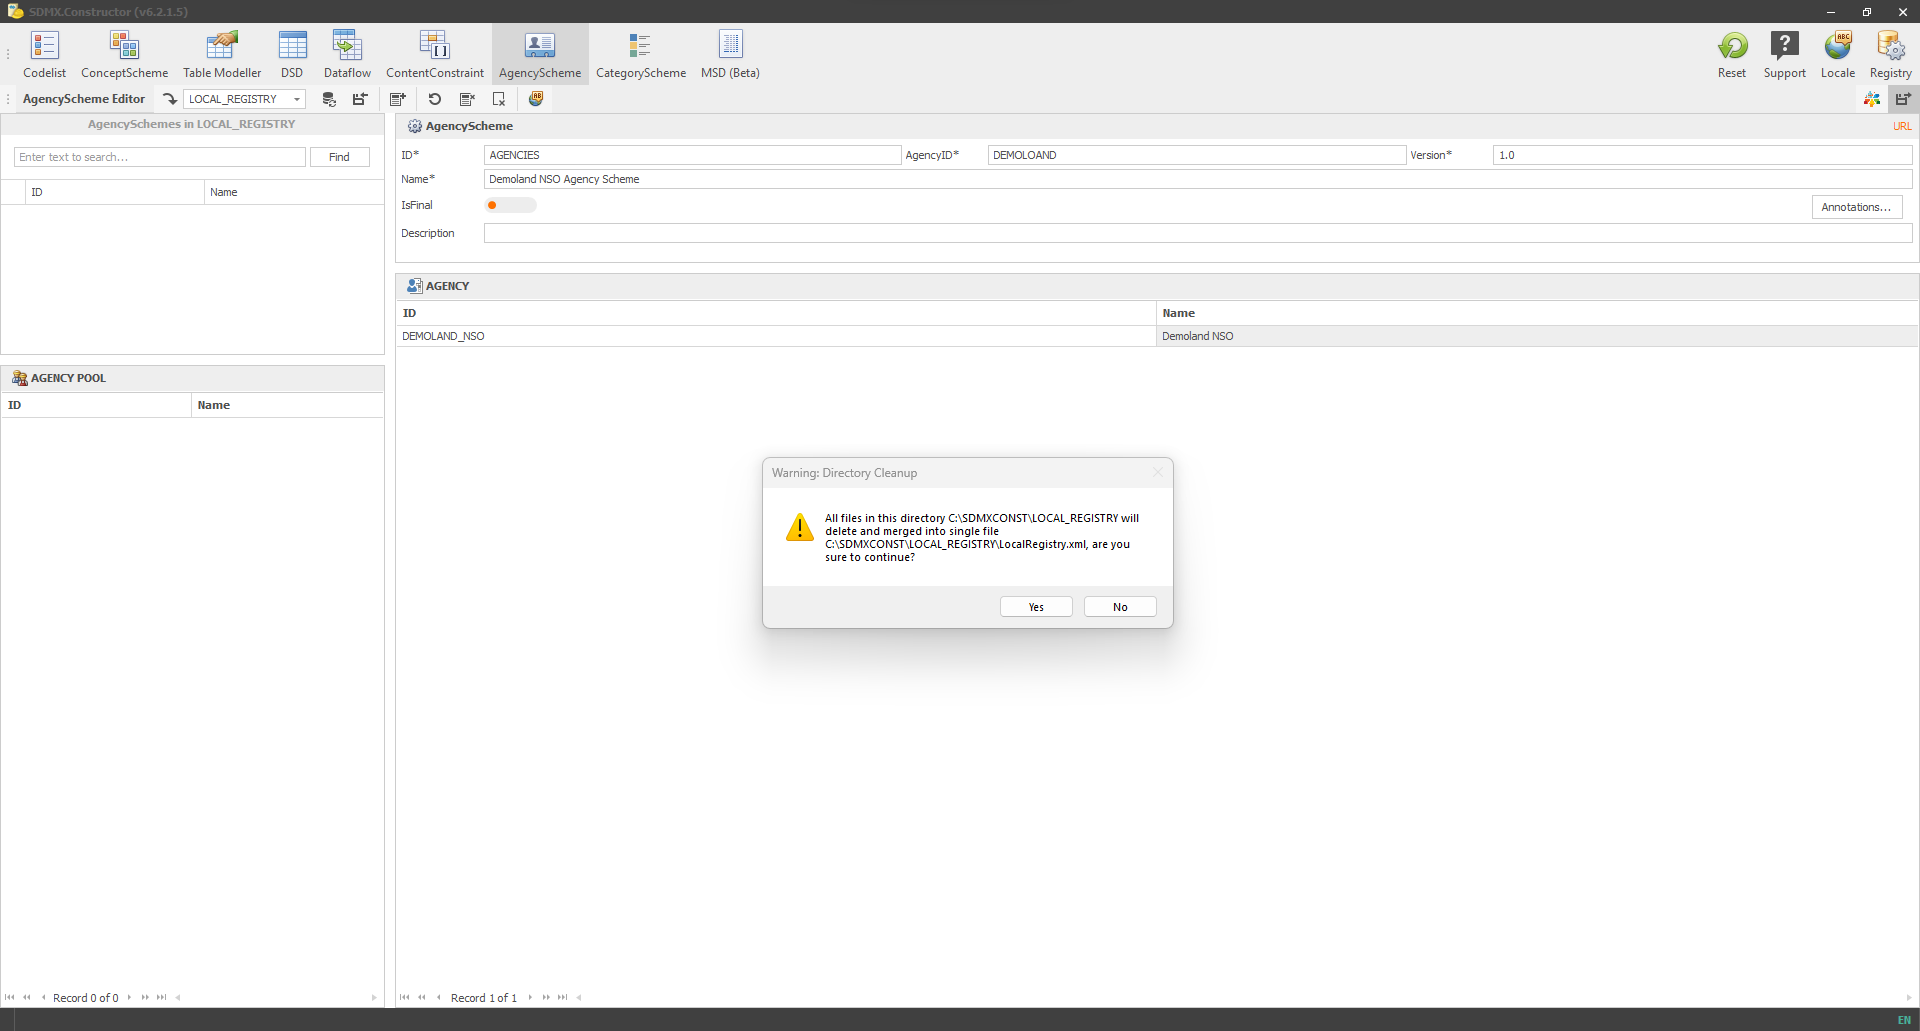
\includegraphics[width=1\linewidth]{./images/image076} \end{center}

\href{images/image076.png}{Click here to enlarge the image}

\begin{itemize}
\tightlist
\item
  Clicking on Yes will create and save an XML file in the folder we created before, as shown below.
\end{itemize}

\begin{center}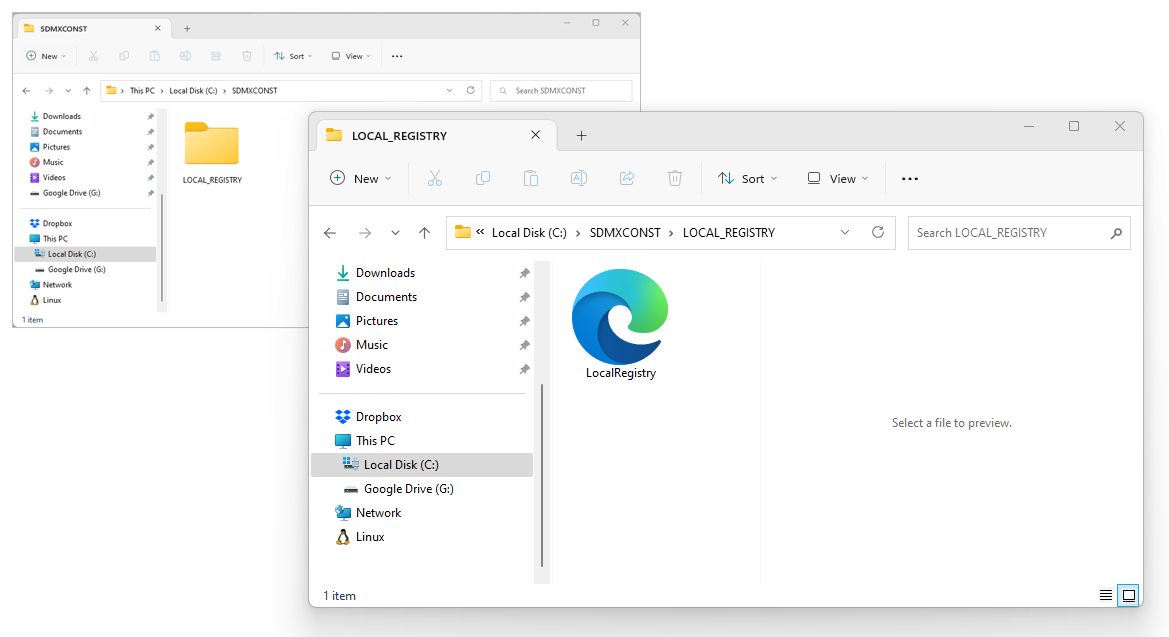
\includegraphics[width=1\linewidth]{./images/image078} \end{center}

\href{images/image078.png}{Click here to enlarge the image}

\begin{itemize}
\tightlist
\item
  Opening the file (LocalRegistry.xml) will show the agency scheme, as shown in the image below.
\end{itemize}

\begin{center}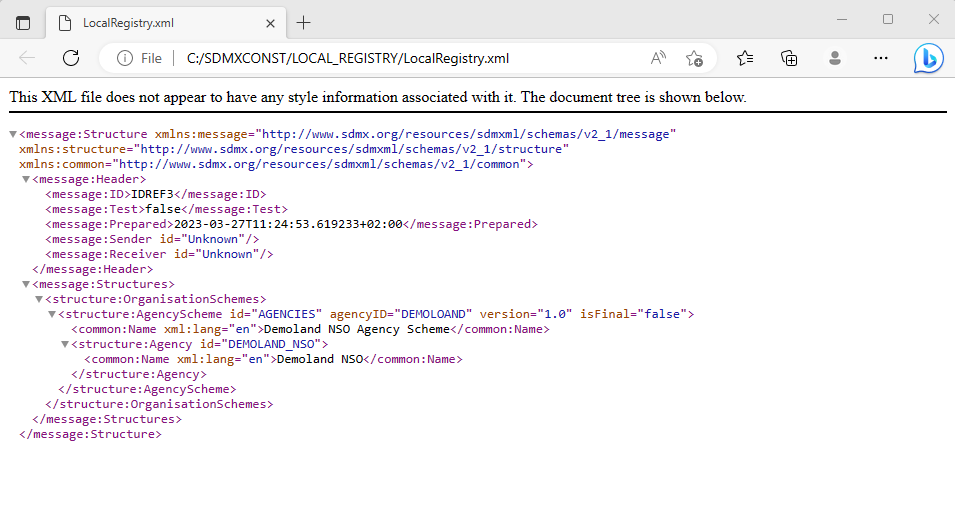
\includegraphics[width=1\linewidth]{./images/image080} \end{center}

\href{images/image080.png}{Click here to enlarge the image}

\hypertarget{creating-conceptscheme}{%
\section{Creating ConceptScheme \& Codelist}\label{creating-conceptscheme}}

We do this in one go. But first, we will upload the Codelist and then the ConceptScheme.

\textbf{Create Codelist:}

\begin{itemize}
\tightlist
\item
  Click on the Codelist button on top and ensure that the folder we created before, LOCAL\_REGISTRY, is selected from the Codelist Editor's `Load from registry' dropdown option, as shown below.
\end{itemize}

\begin{center}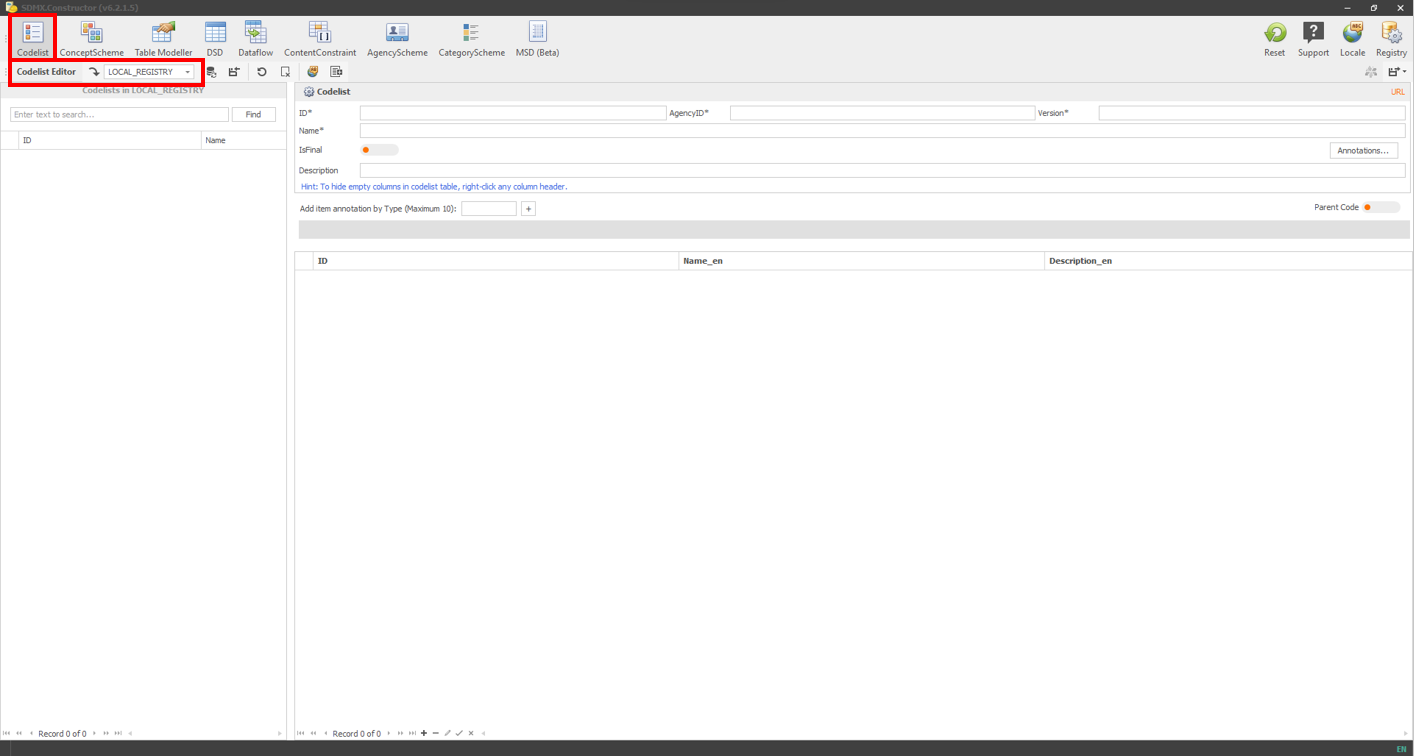
\includegraphics[width=1\linewidth]{./images/image082} \end{center}

\href{images/image082.png}{Click here to enlarge the image}

\begin{itemize}
\tightlist
\item
  Click on the Bulk load button as shown below.
\end{itemize}

\begin{center}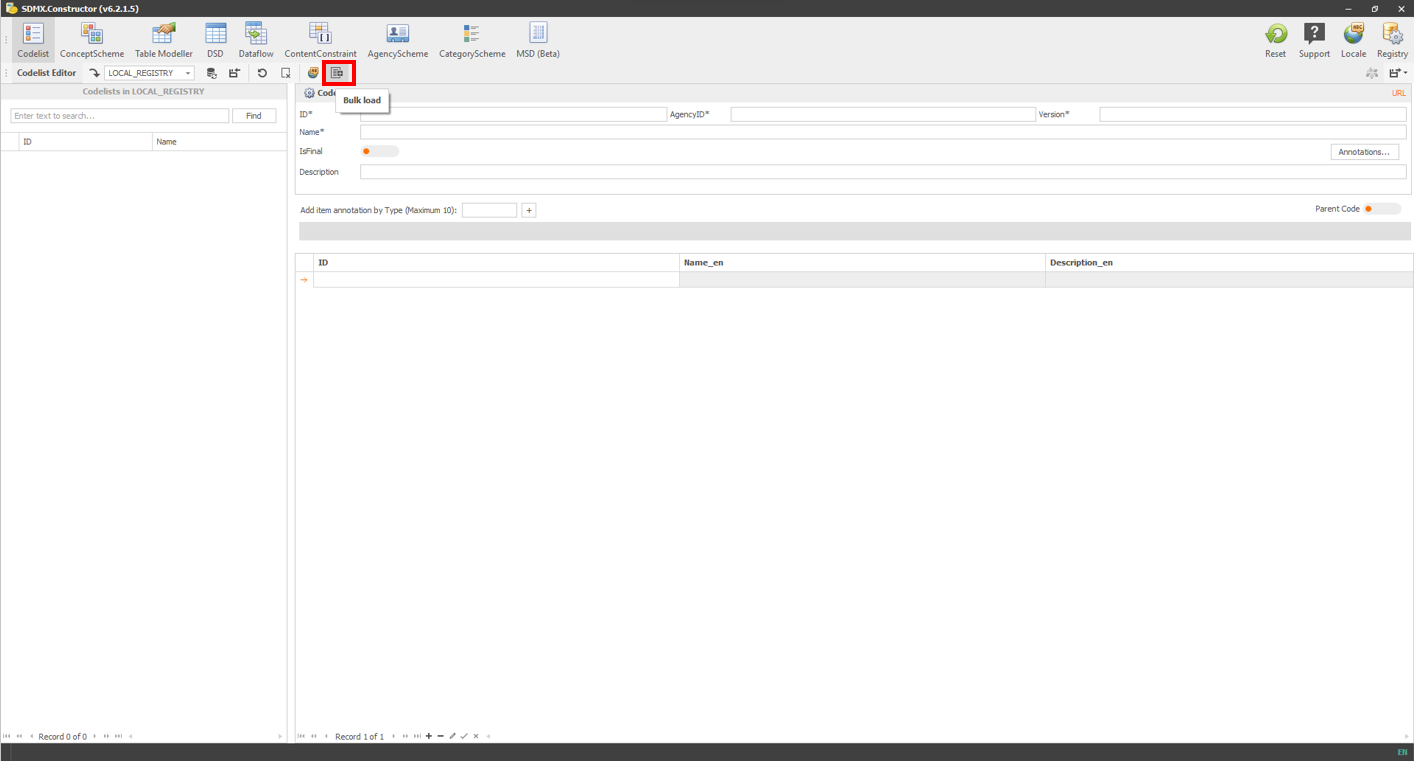
\includegraphics[width=1\linewidth]{./images/image084} \end{center}

\href{images/image084.png}{Click here to enlarge the image}

\begin{itemize}
\tightlist
\item
  It will open up a pop-up window, as shown below.
\end{itemize}

\begin{center}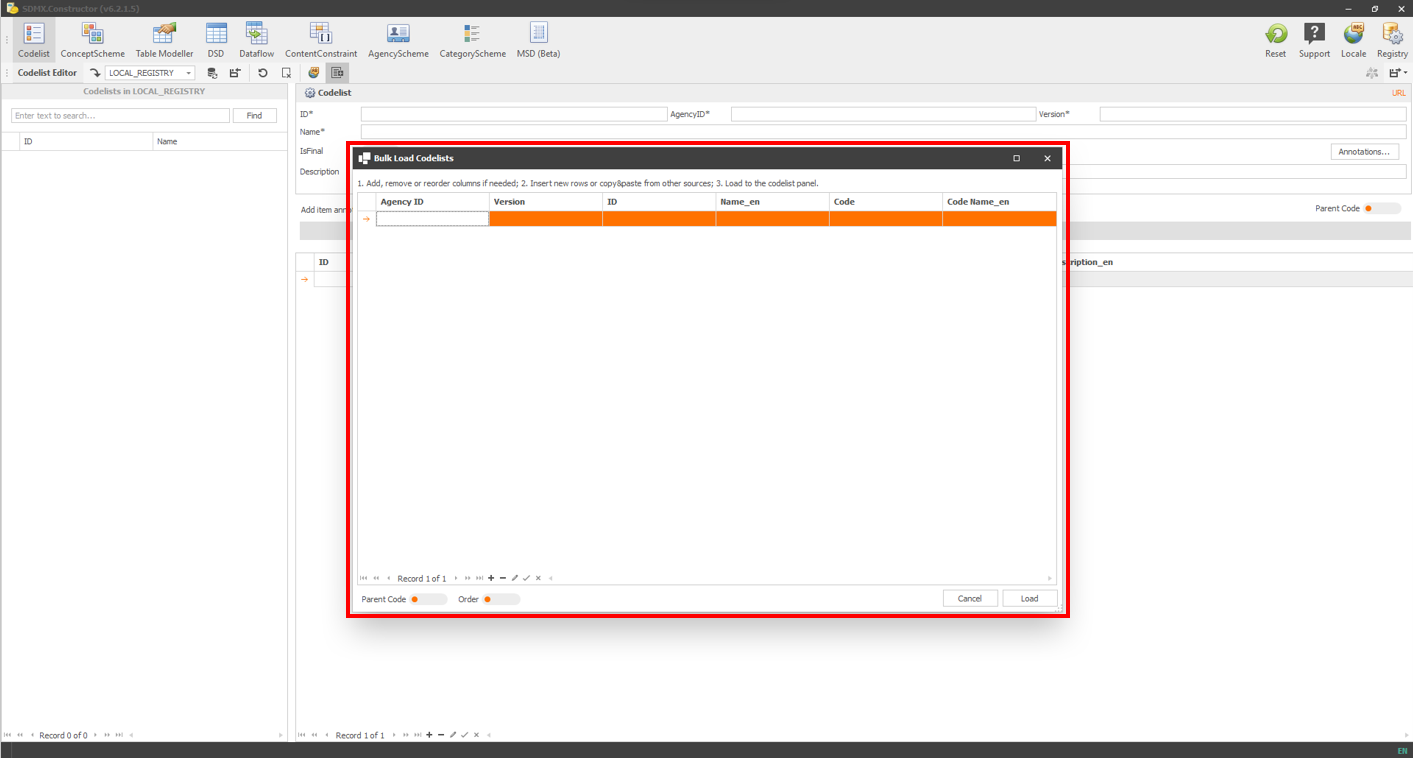
\includegraphics[width=1\linewidth]{./images/image086} \end{center}

\href{images/image086.png}{Click here to enlarge the image}

\begin{itemize}
\tightlist
\item
  Copy the Codelist table (Table: \ref{tab:table44}) we prepared before and paste its contents here. Before pasting, remember to click on the ID column (shown in white in the image below). Then, select the entire row (by clicking on the little arrow (pointing at the right) at the beginning of the rows).
\end{itemize}

\begin{center}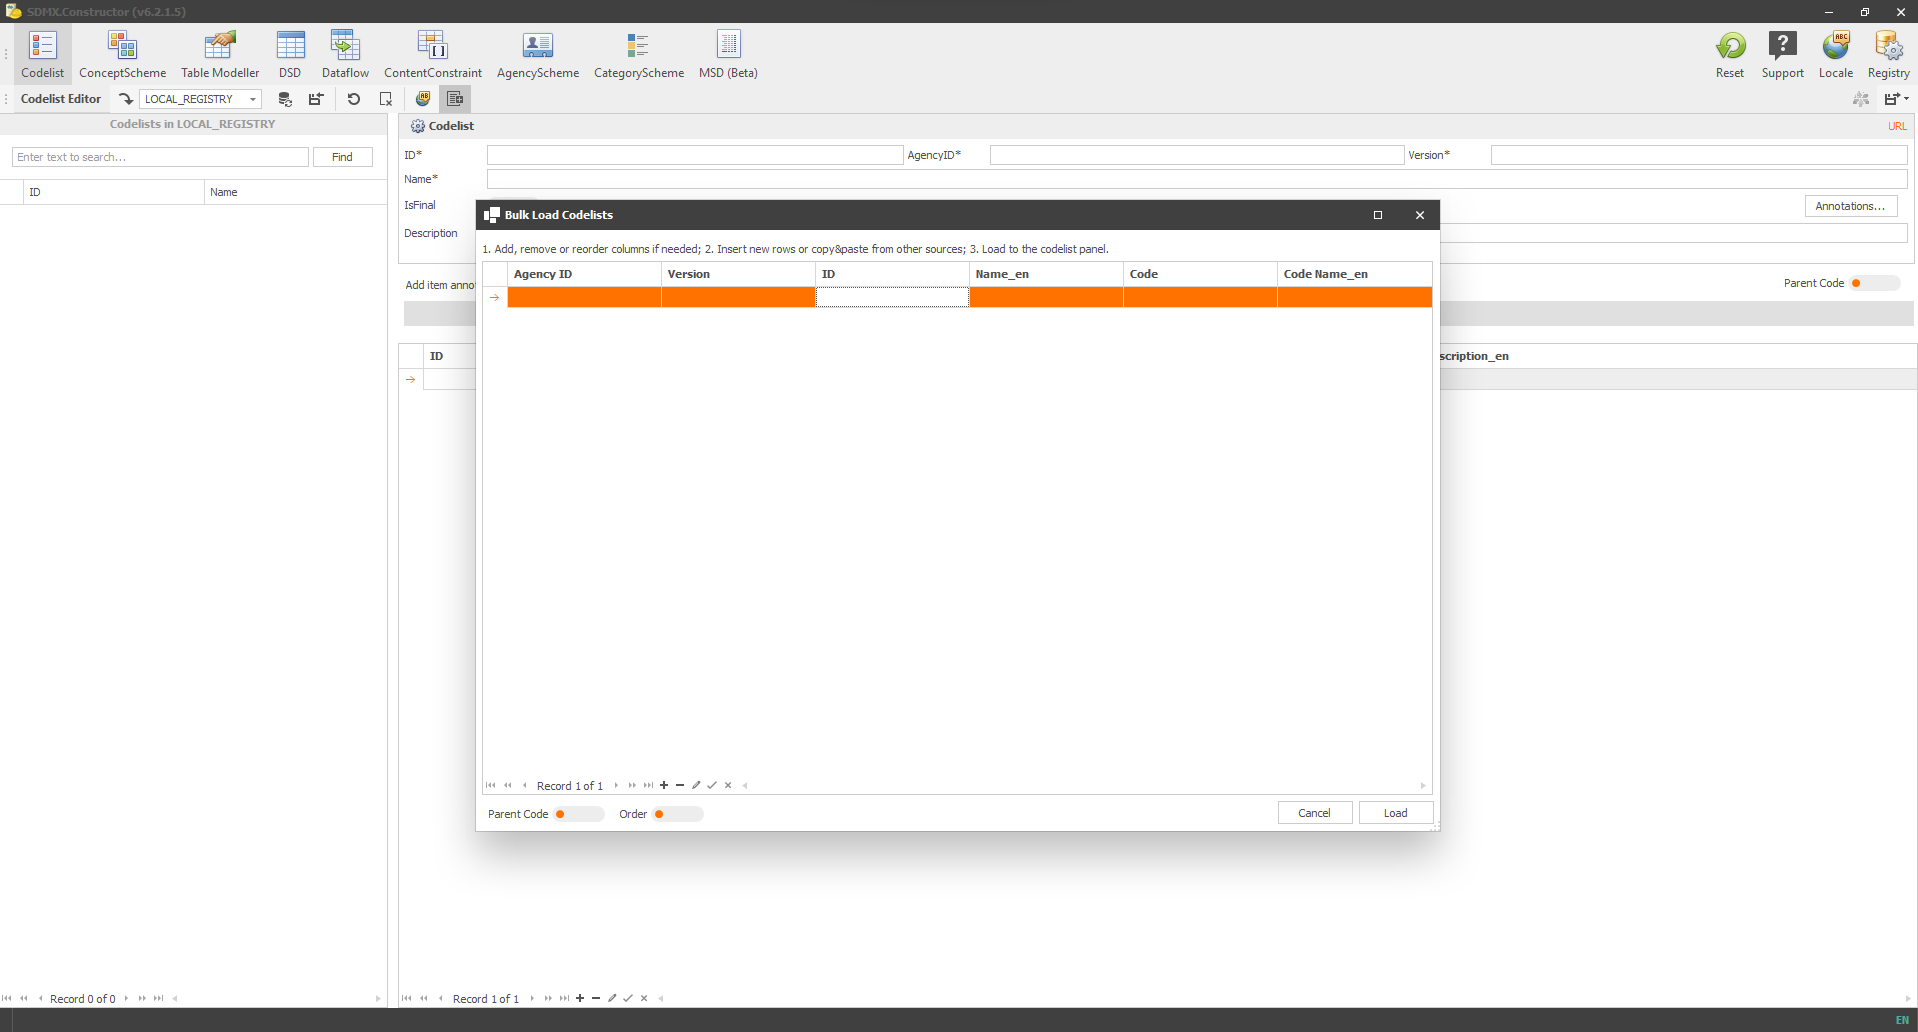
\includegraphics[width=1\linewidth]{./images/image088} \end{center}

\href{images/image088.png}{Click here to enlarge the image}

\begin{itemize}
\tightlist
\item
  After pasting, remember to delete the header row. You can do this by selecting the entire row (by clicking again the little arrow pointing at the right at the beginning of the rows) and clicking the button (``-'') below, as indicated by a downward red arrow.
\end{itemize}

\begin{center}\includegraphics[width=1\linewidth]{./images/image090} \end{center}

\href{images/image090.png}{Click here to enlarge the image}

\begin{itemize}
\tightlist
\item
  Enter the Agency ID and Version on the top row as DEMOLAND\_NSO and 1.0, respectively, as shown below. If only the top row contains entries (DEMOLAND\_NSO and 1.0) and the rest is empty, it implies that the Agency ID and Version are repeated for each row.
\end{itemize}

\begin{center}\includegraphics[width=1\linewidth]{./images/image092} \end{center}

\href{images/image092.png}{Click here to enlarge the image}

\begin{itemize}
\tightlist
\item
  Click on Load, as shown below.
\end{itemize}

\begin{center}\includegraphics[width=1\linewidth]{./images/image094} \end{center}

\href{images/image094.png}{Click here to enlarge the image}

\begin{itemize}
\tightlist
\item
  After the loading, this is how it would look (as shown below).
\end{itemize}

\begin{center}\includegraphics[width=1\linewidth]{./images/image096} \end{center}

\href{images/image096.png}{Click here to enlarge the image}

\begin{itemize}
\tightlist
\item
  Clicking on any item on this list will show the details on the right pane, as shown below.
\end{itemize}

\begin{center}\includegraphics[width=1\linewidth]{./images/image098} \end{center}

\href{images/image098.png}{Click here to enlarge the image}

\textbf{Create ConceptScheme:}

\begin{itemize}
\tightlist
\item
  Click on the ConceptScheme button on top and ensure that the folder we created before, LOCAL\_REGISTRY, is selected from the ConceptScheme Editor's `Load from registry' dropdown option, as shown below.
\end{itemize}

\begin{center}\includegraphics[width=1\linewidth]{./images/image100} \end{center}

\href{images/image100.png}{Click here to enlarge the image}

\begin{itemize}
\tightlist
\item
  Click on the Bulk load button, as shown below.
\end{itemize}

\begin{center}\includegraphics[width=1\linewidth]{./images/image102} \end{center}

\href{images/image102.png}{Click here to enlarge the image}

\begin{itemize}
\tightlist
\item
  It will open up a pop-up window, as shown below.
\end{itemize}

\begin{center}\includegraphics[width=1\linewidth]{./images/image104} \end{center}

\href{images/image104.png}{Click here to enlarge the image}

\begin{itemize}
\tightlist
\item
  Copy the ConceptScheme table (Table: \ref{tab:table43}) we prepared before and paste its contents here. Before pasting, remember to click on the ID column and select the entire row (by clicking on the little arrow at the beginning of the rows).
\end{itemize}

\begin{center}\includegraphics[width=1\linewidth]{./images/image106} \end{center}

\href{images/image106.png}{Click here to enlarge the image}

\begin{itemize}
\tightlist
\item
  After pasting, remember to delete the header row by selecting the entire row and using the button (``-'') below, as indicated by a downward red arrow.
\end{itemize}

\begin{center}\includegraphics[width=1\linewidth]{./images/image108} \end{center}

\href{images/image108.png}{Click here to enlarge the image}

\begin{itemize}
\tightlist
\item
  Click on Load, as shown below.
\end{itemize}

\begin{center}\includegraphics[width=1\linewidth]{./images/image110} \end{center}

\href{images/image110.png}{Click here to enlarge the image}

\begin{itemize}
\tightlist
\item
  After loading, the concepts will be visible in the CONCEPT POOL, as shown below.
\end{itemize}

\begin{center}\includegraphics[width=1\linewidth]{./images/image112} \end{center}

\href{images/image112.png}{Click here to enlarge the image}

\begin{itemize}
\tightlist
\item
  Move all the concepts from the CONCEPT POOL to the CONCEPT pane by selecting all (ctrl + a), then dragging and dropping. After the move, it would look like the following.
\end{itemize}

\begin{center}\includegraphics[width=1\linewidth]{./images/image114} \end{center}

\href{images/image114.png}{Click here to enlarge the image}

\begin{itemize}
\tightlist
\item
  After moving the concepts, enter the details: (ID: CS\_DEMOLAND\_NSO, AgencyID: DEMOLAND\_NSO, Version: 1.0, and Name: Concept Scheme of Demoland NSO) for the ConceptScheme, as shown below.
\end{itemize}

\begin{center}\includegraphics[width=1\linewidth]{./images/image116} \end{center}

\href{images/image116.png}{Click here to enlarge the image}

\begin{itemize}
\tightlist
\item
  Then, click the `Save with descendants' from the save option as shown below. This option, `Save with descendants,' will save the concept scheme with the codelist.
\end{itemize}

\begin{center}\includegraphics[width=1\linewidth]{./images/image118} \end{center}

\href{images/image118.png}{Click here to enlarge the image}

\begin{itemize}
\tightlist
\item
  A pop-up message will ask to save the XML file in the folder (LOCAL\_REGISTRY) we created before. Click on Save to save the file.
\end{itemize}

\begin{center}\includegraphics[width=1\linewidth]{./images/image123} \end{center}

\href{images/image123.png}{Click here to enlarge the image}

\begin{itemize}
\tightlist
\item
  After clicking Save, the tool will ask the question to merge files. Select Yes.
\end{itemize}

\begin{center}\includegraphics[width=1\linewidth]{./images/image125} \end{center}

\href{images/image125.png}{Click here to enlarge the image}

\begin{itemize}
\tightlist
\item
  A confirmation message will appear for a short time at the bottom right corner, as shown below.
\end{itemize}

\begin{center}\includegraphics[width=1\linewidth]{./images/image127} \end{center}

\href{images/image127.png}{Click here to enlarge the image}

\begin{itemize}
\tightlist
\item
  After that, if you go to the file's location, you will see the XML file created, as shown below.
\end{itemize}

\begin{center}\includegraphics[width=0.5\linewidth]{./images/image129} \end{center}

\href{images/image129.png}{Click here to enlarge the image}

\begin{itemize}
\tightlist
\item
  Opening the XML file will show the details containing, AgencyScheme, ConceptScheme and Codelists.
\end{itemize}

\hypertarget{creating-dsd}{%
\section{Creating DSD, Dataflow, ContentConstraint and CategoryScheme}\label{creating-dsd}}

Recalling our two initial tables (Table: \ref{tab:table41} and Table: \ref{tab:table42}), we will now generate DSDs, ContentConstraints and Dataflows. We will also create a CategoryScheme. We can create all these artefacts through the \protect\hyperlink{table-modeller}{Table Modeller} option in the SDMX Constructor.

The Table Modeller offers the functionality to design statistical tables with an intuitive user interface to generate the SDMX artefacts that model it.

\begin{itemize}
\tightlist
\item
  Click on the Table Modeller button on top and ensure that the folder we created before, LOCAL\_REGISTRY, is selected from the Table Modeller Editor's `Load from registry' dropdown option, as shown below.
\end{itemize}

\begin{center}\includegraphics[width=1\linewidth]{./images/image130} \end{center}

\href{images/image130.png}{Click here to enlarge the image}

\begin{itemize}
\tightlist
\item
  You will notice the concept scheme we created before, as highlighted below.
\end{itemize}

\begin{center}\includegraphics[width=1\linewidth]{./images/image132} \end{center}

\href{images/image132.png}{Click here to enlarge the image}

\begin{itemize}
\tightlist
\item
  Double-clicking the concept scheme will move it to the CONCEPT POOL, as shown below.
\end{itemize}

\begin{center}\includegraphics[width=1\linewidth]{./images/image134} \end{center}

\href{images/image134.png}{Click here to enlarge the image}

\begin{itemize}
\item
  Now, you can select the concepts in the CONCEPT POOL, then drag and drop them into various spaces (Constant Dimensions, Header, Side, Measures \& Observation Attributes and Footnotes \& Table Attributes) on the right pane. The logic driving where to drop each concept comes from our original tables (Table: \ref{tab:table41} and Table: \ref{tab:table42}).
\item
  For Table \ref{tab:table41} (Unemployment Rate by sex and region), the following distribution will be representative.
\end{itemize}

\begin{center}\includegraphics[width=1\linewidth]{./images/image136} \end{center}

\href{images/image136.png}{Click here to enlarge the image}

\begin{itemize}
\tightlist
\item
  We can now apply two constraints: one for the indicator's name and the other for the unit of measure. The indicator's name will be the Unemployment Rate, which we can select by double-clicking the moved indicator concept as shown below.
\end{itemize}

\begin{center}\includegraphics[width=1\linewidth]{./images/image138} \end{center}

\href{images/image138.png}{Click here to enlarge the image}

\begin{itemize}
\tightlist
\item
  Another constraint would be the unit of measure. Because it is `rate' (for Table \ref{tab:table41}), double-clicking the moved unit of measure concept would offer the option to select the rate. Select the Rate as shown below.
\end{itemize}

\begin{center}\includegraphics[width=1\linewidth]{./images/image140} \end{center}

\href{images/image140.png}{Click here to enlarge the image}

\begin{itemize}
\tightlist
\item
  Now we add the table information as shown below.
\end{itemize}

\begin{center}\includegraphics[width=1\linewidth]{./images/image142} \end{center}

\href{images/image142.png}{Click here to enlarge the image}

\begin{itemize}
\tightlist
\item
  Then we will hit save (select `Save without descendants'), as shown below.
\end{itemize}

\begin{center}\includegraphics[width=1\linewidth]{./images/image144} \end{center}

\href{images/image144.png}{Click here to enlarge the image}

\begin{itemize}
\tightlist
\item
  After saving, it will show a message as shown below.
\end{itemize}

\begin{center}\includegraphics[width=1\linewidth]{./images/image146} \end{center}

\href{images/image146.png}{Click here to enlarge the image}

\begin{itemize}
\tightlist
\item
  Clicking on Continue will result in a pop-up asking to save the file, as shown below.
\end{itemize}

\begin{center}\includegraphics[width=1\linewidth]{./images/image152} \end{center}

\href{images/image152.png}{Click here to enlarge the image}

\begin{itemize}
\tightlist
\item
  Clicking Save will show this message and ask if the files should be merged.
\end{itemize}

\begin{center}\includegraphics[width=1\linewidth]{./images/image154} \end{center}

\href{images/image154.png}{Click here to enlarge the image}

\begin{itemize}
\tightlist
\item
  Clicking on Yes will merge the file.
\item
  We will repeat the process for Table \ref{tab:table42} (Population outside the labour force by sex and age group (2022)). We can do that by moving Age to the `Side' space (and removing the Geo back to the CONCEPT POOL), changing the constraints for the indicator to `Population outside the labour force' and unit of measure to `Persons', and updating the table information as shown below.
\end{itemize}

\begin{center}\includegraphics[width=1\linewidth]{./images/image156} \end{center}

\href{images/image156.png}{Click here to enlarge the image}

\begin{itemize}
\tightlist
\item
  After hitting the save (Save without descendants) button, the message will read like the one below.
\end{itemize}

\begin{center}\includegraphics[width=1\linewidth]{./images/image158} \end{center}

\href{images/image158.png}{Click here to enlarge the image}

\begin{itemize}
\item
  Proceed with `Continue', `Save', and `Yes' for merge.
\item
  We should see two DSDs, two content constraints and two data flows. \texttt{Remember,\ dataflows\ are\ the\ filtered\ view\ of\ the\ DSDs.}
\end{itemize}

\textbf{Category scheme}

Now, we can create a categorisation scheme. The categorisation could be by topics such as `Unemployment Rate' and `Population outside the labour force'.

\begin{itemize}
\tightlist
\item
  First, we will click the CategoryScheme button and enter the properties (ID: CAS\_BY\_TOPIC, AgencyID: DEMOLAND\_NSO, Version: 1.0 and Name: Categorisation Scheme By Topic) as shown below.
\end{itemize}

\begin{center}\includegraphics[width=1\linewidth]{./images/image160} \end{center}

\href{images/image160.png}{Click here to enlarge the image}

\begin{itemize}
\tightlist
\item
  Click on ``Add New Category'', as shown below.
\end{itemize}

\begin{center}\includegraphics[width=1\linewidth]{./images/image162} \end{center}

\href{images/image162.png}{Click here to enlarge the image}

\begin{itemize}
\tightlist
\item
  It will open a pop-up window, as shown below. Enter the details: ID: UNER (shorthand for Unemployment Rate) and Name: Unemployment Rate.
\end{itemize}

\begin{center}\includegraphics[width=1\linewidth]{./images/image164} \end{center}

\href{images/image164.png}{Click here to enlarge the image}

\begin{itemize}
\tightlist
\item
  Click on the Load ``Dataflows'' button, as shown below.
\end{itemize}

\begin{center}\includegraphics[width=1\linewidth]{./images/image166} \end{center}

\href{images/image166.png}{Click here to enlarge the image}

\begin{itemize}
\tightlist
\item
  It will open another pop-up window to select the dataflow through the Registry.
\end{itemize}

\begin{center}\includegraphics[width=1\linewidth]{./images/image168} \end{center}

\href{images/image168.png}{Click here to enlarge the image}

\begin{itemize}
\tightlist
\item
  Select the Registry (LOCAL\_REGISTRY), then the dataflow, and press Apply as shown below.
\end{itemize}

\begin{center}\includegraphics[width=1\linewidth]{./images/image170} \end{center}

\href{images/image170.png}{Click here to enlarge the image}

\begin{itemize}
\tightlist
\item
  A message will appear as shown below.
\end{itemize}

\begin{center}\includegraphics[width=1\linewidth]{./images/image172} \end{center}

\href{images/image172.png}{Click here to enlarge the image}

\begin{itemize}
\tightlist
\item
  Clicking the OK button will lead you to the following window.
\end{itemize}

\begin{center}\includegraphics[width=1\linewidth]{./images/image174} \end{center}

\href{images/image174.png}{Click here to enlarge the image}

\begin{itemize}
\tightlist
\item
  As shown below, move (dragging and dropping) the dataflow to the `attached dataflows' space.
\end{itemize}

\begin{center}\includegraphics[width=1\linewidth]{./images/image176} \end{center}

\href{images/image176.png}{Click here to enlarge the image}

\begin{itemize}
\tightlist
\item
  Clicking ``Apply'' in that pop-up will take you to the following window, showing the entry into the CATEGORY POOL.
\end{itemize}

\begin{center}\includegraphics[width=1\linewidth]{./images/image178} \end{center}

\href{images/image178.png}{Click here to enlarge the image}

\begin{itemize}
\tightlist
\item
  Move it to the right pane, as shown below.
\end{itemize}

\begin{center}\includegraphics[width=1\linewidth]{./images/image180} \end{center}

\href{images/image180.png}{Click here to enlarge the image}

\begin{itemize}
\tightlist
\item
  Then hit Save (Save without descendants), and it will show the pop-up windows to ensure the location where it saves the file, as shown below.
\end{itemize}

\begin{center}\includegraphics[width=1\linewidth]{./images/image182} \end{center}

\href{images/image182.png}{Click here to enlarge the image}

\begin{itemize}
\tightlist
\item
  Clicking on Save will ask the confirmation to merge the file. Select Yes.
\item
  Repeat the process for the other category, `Population outside the labour force'. The final view would be as follows:
\end{itemize}

\begin{center}\includegraphics[width=1\linewidth]{./images/image184} \end{center}

\href{images/image184.png}{Click here to enlarge the image}

\begin{itemize}
\tightlist
\item
  The XML file (by going to the location of the folder we created before and opening the XML file) would be like the one below.
\end{itemize}

\begin{center}\includegraphics[width=1\linewidth]{./images/image186} \end{center}

\href{images/image186.png}{Click here to enlarge the image}

\hypertarget{uploading-xml}{%
\section{Uploading XML file to the DLM}\label{uploading-xml}}

You can upload the XML file containing the SDMX artefacts to the .Stat Data Lifecycle Manager (DLM). The DLM could be on the cloud or local computer (Localhost). Here is one case illustrated where we upload the XML file we created and saved using the SDMX Constructor in a folder to a locally hosted instance of the DLM.

\begin{quote}
\textbf{Note on artefact versioning}: Artefact versioning is crucial for managing SDMX artefacts, as it prevents conflicts when uploading structures to the DLM. This is especially important when multiple users work on the same artefact simultaneously or when updating artefacts over time. You may recall the usual place (in the right corner of the respective windows) to enter the version number in the user interface for creating or modifying artefacts in the SDMX Constructor.
\end{quote}

\begin{itemize}
\tightlist
\item
  Start the DLM. Configured as localhost, it will look like the following.
\end{itemize}

\begin{center}\includegraphics[width=1\linewidth]{./images/image188} \end{center}

\href{images/image188.png}{Click here to enlarge the image}

\begin{itemize}
\tightlist
\item
  Login using your credentials.
\end{itemize}

\begin{center}\includegraphics[width=1\linewidth]{./images/image190} \end{center}

\href{images/image190.png}{Click here to enlarge the image}

\begin{itemize}
\tightlist
\item
  Click on the `Upload structures' button as shown below:
\end{itemize}

\begin{center}\includegraphics[width=1\linewidth]{./images/image192} \end{center}

\href{images/image192.png}{Click here to enlarge the image}

\begin{itemize}
\tightlist
\item
  Click on `Add files' as shown below.
\end{itemize}

\begin{center}\includegraphics[width=1\linewidth]{./images/image194} \end{center}

\href{images/image194.png}{Click here to enlarge the image}

\begin{itemize}
\tightlist
\item
  Select the XML file we created before from the folder as shown below.
\end{itemize}

\begin{center}\includegraphics[width=1\linewidth]{./images/image196} \end{center}

\href{images/image196.png}{Click here to enlarge the image}

\begin{itemize}
\tightlist
\item
  After adding the file, select the `demo-design' space, as shown below.
\end{itemize}

\begin{center}\includegraphics[width=1\linewidth]{./images/image198} \end{center}

\href{images/image198.png}{Click here to enlarge the image}

\begin{itemize}
\tightlist
\item
  Click upload as shown below.
\end{itemize}

\begin{center}\includegraphics[width=1\linewidth]{./images/image200} \end{center}

\href{images/image200.png}{Click here to enlarge the image}

\begin{itemize}
\tightlist
\item
  As shown below, the green background and the message will indicate the successful XML file upload.
\end{itemize}

\begin{center}\includegraphics[width=1\linewidth]{./images/image202} \end{center}

\href{images/image202.png}{Click here to enlarge the image}

\begin{itemize}
\tightlist
\item
  Clicking the Home icon will take you to the following interface.
\end{itemize}

\begin{center}\includegraphics[width=1\linewidth]{./images/image204} \end{center}

\href{images/image204.png}{Click here to enlarge the image}

\begin{itemize}
\tightlist
\item
  Here, selecting the options on the left navigation panel will show the artefacts on the main pane, as shown below.
\end{itemize}

\begin{center}\includegraphics[width=1\linewidth]{./images/image206} \end{center}

\href{images/image206.png}{Click here to enlarge the image}

\hypertarget{connecting-to}{%
\section{Connecting to an SDMX registry}\label{connecting-to}}

SDMX Constructor can also connect to a new SDMX registry (such as .Stat DLM) directly, and users can directly pull or push (perhaps after editing) artefacts from the SDMX Constructor.

\begin{itemize}
\tightlist
\item
  After launching the SDMX Constructor, click on the Registry, as shown below.
\end{itemize}

\begin{center}\includegraphics[width=1\linewidth]{./images/image208} \end{center}

\href{images/image208.png}{Click here to enlarge the image}

\begin{itemize}
\tightlist
\item
  The default value you can see is as follows.
\end{itemize}

\begin{center}\includegraphics[width=1\linewidth]{./images/image210} \end{center}

\href{images/image210.png}{Click here to enlarge the image}

\begin{itemize}
\tightlist
\item
  Change the default values for Registry Name and Base URL. For Registry Name, you can choose a name of your choice. For example, Registry Name is DLM, and for the Base URL, the localhost configuration is already specified (by default, it will be \url{http://127.0.0.1/rest/}).
\end{itemize}

\begin{center}\includegraphics[width=1\linewidth]{./images/image212} \end{center}

\href{images/image212.png}{Click here to enlarge the image}

\begin{itemize}
\tightlist
\item
  Clicking on Save will show the message shown below. Click on OK.
\end{itemize}

\begin{center}\includegraphics[width=1\linewidth]{./images/image214} \end{center}

\href{images/image214.png}{Click here to enlarge the image}

\begin{itemize}
\tightlist
\item
  Once the Registry is set, select it from the `Load from registry' option, as shown below.
\end{itemize}

\begin{center}\includegraphics[width=1\linewidth]{./images/image216} \end{center}

\href{images/image216.png}{Click here to enlarge the image}

Doing this syncs the artefacts. For instance, you can see the dataflows in SDMX Constructor populated from the DLM. However, pushing any new entry (in this case, let's say, a new dataflow) to DLM would require the credentials for the DLM.

\begin{itemize}
\tightlist
\item
  From the concepts obtained from the DLM, as shown below, let's create a new data flow.
\end{itemize}

\begin{center}\includegraphics[width=1\linewidth]{./images/image218} \end{center}

\href{images/image218.png}{Click here to enlarge the image}

\begin{itemize}
\tightlist
\item
  Move the concepts around and enter table details as shown below.
\end{itemize}

\begin{center}\includegraphics[width=1\linewidth]{./images/image220} \end{center}

\href{images/image220.png}{Click here to enlarge the image}

\begin{itemize}
\tightlist
\item
  Apply the content constraints as shown below.
\end{itemize}

\begin{center}\includegraphics[width=1\linewidth]{./images/image222} \end{center}

\href{images/image222.png}{Click here to enlarge the image}

\begin{itemize}
\tightlist
\item
  Then click on the Push to DLM button, as shown below.
\end{itemize}

\begin{center}\includegraphics[width=1\linewidth]{./images/image224} \end{center}

\href{images/image224.png}{Click here to enlarge the image}

\begin{itemize}
\tightlist
\item
  Select `Push without descendants'.
\end{itemize}

\begin{center}\includegraphics[width=1\linewidth]{./images/image226} \end{center}

\href{images/image226.png}{Click here to enlarge the image}

\begin{itemize}
\tightlist
\item
  After entering the credentials for the DLM, push, and you will see a message like the one below.
\end{itemize}

\begin{center}\includegraphics[width=1\linewidth]{./images/image228} \end{center}

\href{images/image228.png}{Click here to enlarge the image}

\begin{itemize}
\tightlist
\item
  After you have pressed the Continue button, you will see the following. The message mentions what has changed and what has not. In this case, it notes no DSD change, but one data flow and a content constraint have been created.
\end{itemize}

\begin{center}\includegraphics[width=1\linewidth]{./images/image230} \end{center}

\href{images/image230.png}{Click here to enlarge the image}

\begin{itemize}
\tightlist
\item
  Click on OK and go to the DLM. In the DLM, clicking on the dataflow would show the additional dataflow added directly through the SDMX Constructor to the DLM, as shown below.
\end{itemize}

\begin{center}\includegraphics[width=1\linewidth]{./images/image232} \end{center}

\href{images/image232.png}{Click here to enlarge the image}

\hypertarget{special-topics}{%
\chapter{Special Topics}\label{special-topics}}

\hypertarget{annotations}{%
\section{Annotations}\label{annotations}}

\hypertarget{table-modeller}{%
\section{Table Modeller}\label{table-modeller}}

The Table Modeller functionality supports designing statistical tables using an intuitive user interface that generates the SDMX artefacts that model it. The interface is designed to use statistical terms to name objects, hiding the SDMX artefact names wherever possible, making it user-friendly and accessible.

By understanding the user interface (as shown below), the users of the Table Modeller functionality in SDMX Constructor can easily create statistical tables that generate the SDMX artefacts. Note that the table is a view of a container, which defines how the data will be stored.

\begin{center}\includegraphics[width=1\linewidth]{./images/image234} \end{center}

\href{images/image234.png}{Click here to enlarge the image}

The placeholders provided in the Table Modeller interface help users understand and include different concepts in the table and create well-defined SDMX artefacts.

A table in SDMX parlance represents a Dataflow, has a title, and comprises concepts (SDMX CONCEPTS) that take different roles in the table. The Table Modeller interface has various placeholders for the concepts, which are:

\begin{itemize}
\item
  \textbf{Constant Dimensions:} A placeholder for SDMX CONCEPT type DIMENSIONS that remain constant across the table, such as indicator or measure and frequency.
\item
  \textbf{Header:} A placeholder for SDMX CONCEPT type DIMENSIONS that appear at the top of the table, such as time-period.
\item
  \textbf{Side:} A placeholder for SDMX CONCEPT type DIMENSIONS that appear on the left-hand side of the table. It can contain dimensions such as Age or Region (urban/rural).
\item
  \textbf{Measure \& Observation Attributes:} A placeholder for observation values (or primary measure) and SDMX CONCEPT type ATTRIBUTES attached at the observation level, such as DECIMALS.
\item
  \textbf{Footnotes \& Table Attributes:} A placeholder for SDMX CONCEPT type ATTRIBUTES such as `free text' notes and `source' attached at the dataset level.
\end{itemize}

\textbf{Using the Table Modeller}

\begin{itemize}
\item
  You can ``drag-and-drop'' concepts from the CONCEPT POOL on the left panel to the different areas/spaces/placeholders on the right panel.
\item
  The concepts dropped in the ``Side'', ``Header'', and ``Measure \& Observation Attributes'' areas will become DIMENSIONS. Note that the relative position of the concept in the area is relevant.
\item
  Concepts dropped in ``Constant Dimensions'' will also be DIMENSIONS, but the user will have to select one (and only one) item from each DIMENSION'S Codelist, which will be assigned to it (as ContentConstraint).
\item
  Concepts dropped in the ``Measure \& Observation Attributes'' area, and the ``Footnotes \& Table Attributes'' area will become ATTRIBUTES, the former attached at the Observation level and the latter at the Dataset level.
\item
  The outputs of the Table Modeller are the artefacts needed to represent in SDMX the table design.
\end{itemize}

\hypertarget{translations-using-google-apideepl}{%
\section{Translations using Google API/DeepL}\label{translations-using-google-apideepl}}

  \bibliography{book.bib,packages.bib}

\end{document}
